\chapter{Implementation}
\label{ch:implementation}

\section{The Projected Grid}
\label{sec_projected_grid}
The projected grid is based on a simple concept: in order to achieve an
uniform distribution of details on the image plane, a uniformly spaced grid is
created in post-perspective space and transformed back to world space.
Figure~\ref{fig:projectedgrid} illustrates the difference between a classic
world space approach and the projected grid.
\begin{figure}[h]
\centering
\subbottom[Classic]
{
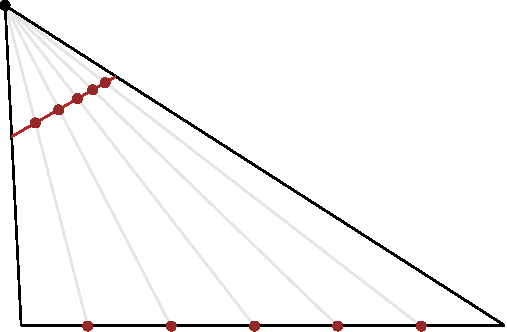
\includegraphics[scale=0.75]{figures/ProjectedGridVsWorldSpace.pdf}
\label{fig:subfigprojgrid1}
}
\subbottom[Projected Grid]
{
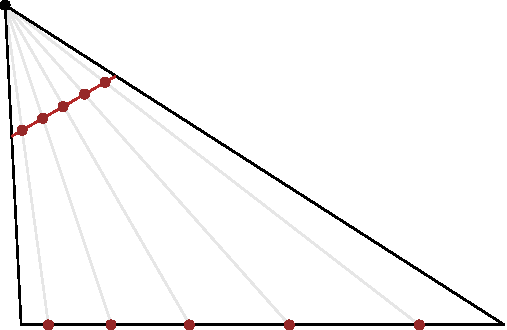
\includegraphics[scale=0.75]{figures/ProjectedGridUniform.pdf}
\label{fig:subfigprojgrid2}
}
\caption{The image on the left shows an uniform grid in worldspace,
its projection onto the image plane is not uniformly spaced though.
The image on the right on the other hand depicts an uniform grid on
the image plane and its associated non-uniform spaced worldspace
positions.}
\label{fig:projectedgrid}
\end{figure}

% The algorithm used for the projected grid can be broken down into the following
% steps:
% \begin{itemize}
%  \item create a uniformly spaced grid orthogonal to the viewer using normalised
% device coordinates
%  \item transform the grid to worldspace
%  \item project the grid onto the desired base plane
%  \item apply height displacement
%  \item run the grid through the rendering pipeline as usual
% \end{itemize}

\subsection{Coordinate Systems}
\label{sec:coordinate_systems}
Let $\mvec{x}$ be a vector representing the three dimensional carthesian
world space coordinate of a vertex, then
\begin{equation}
 \mvec{w} = \transpose{(\mvecx{x}, \mvecy{x}, \mvecz{x}, 1)}
\end{equation}
where $\mvec{w}$ is a homogeneous world space coordinate of $\mvec{x}$.
Let $\mmat{V}$ be the view matrix and $\mmat{P}$ the projection matrix, then
\begin{equation}
\label{eq:ws_to_cs}
 \mvec{c} = \mmat{P} \mmat{V} \mvec{w}
\end{equation}
where $\mvec{c}$ is the \textit{clip space} coordinate of $\mvec{w}$. For $\mvec{c}$ to
be inside the view frustum defined by $\mmat{P}$, $\mvec{c}$ is required to
meet the following condition
\begin{equation}
\label{eq:cs_bounds}
 \mvecx{c}, \mvecy{c}, \mvecz{c} \in \interval{-\mvecw{c}}{\mvecw{c}}
\end{equation}
where $\mvecw{c}$ is the homogeneous component of $\mvec{c}$. Next, clip space
vertex $\mvec{c}$ is transformed by the \textit{perspective division} as follows
\begin{equation}
\label{eq:cs_to_ndc}
 \mvec{n} = \frac{1}{\mvecw{c}}\transpose{(\mvecx{c}, \mvecy{c}, \mvecz{c})}
\end{equation}
where $\mvec{n}$ corresponds to the \textit{normalised device coordinate},
\textit{NDC} in short, of $\mvec{c}$.
%
%
\begin{figure}
\centering
\subbottom[View Frustum]
{
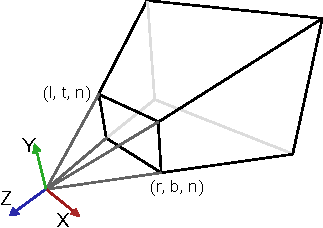
\includegraphics[width=0.4\textwidth]{figures/ProjectiveFrustum.pdf}
\label{fig:subfig_proj_frustum}
}
\subbottom[Canonical view volume]
{
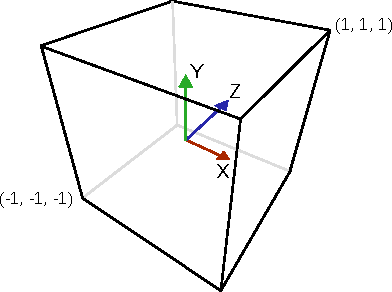
\includegraphics[width=0.4\textwidth]{figures/CanonicalCube.pdf}
\label{fig:subfig_canonical_view_volume}
}
\caption{Left: An example view frustum in view space. Right: The same view frustum
after applying projection and perspective division.}
\label{fig:proj_frustum_ndc}
\end{figure}
%
%
As one can see, equations~\ref{eq:cs_bounds}
and~\ref{eq:cs_to_ndc} imply
\begin{equation}
\label{eq:ndc_bounds}
 \mvecx{n}, \mvecy{n}, \mvecz{n} \in \interval{-1}{1}
\end{equation}
which defines the space NDC reside in, namely the \textit{canonical view volume},
see Figure~\ref{fig:proj_frustum_ndc}.\\


The projected grid, on the other hand, starts inside the canonical view volume
and needs to transform vertices back to world space. Let $\mvec{n}$ be the
normalised device coordinate of a vertex, then
\begin{equation}
\label{eq:ndc_to_cs}
 \mvec{c} = \transpose{(\mvecx{n}, \mvecy{n}, \mvecz{n}, 1)}
\end{equation}
where $\mvec{c}$ is a valid representation of $\mvec{n}$ in clip space. One may choose
a value for $\mvecw{c}$ different from $1$, making it necessary to scale $\mvecx{n}$,
$\mvecy{n}$ and $\mvecz{n}$ accordingly. Again, let $\mmat{V}$ be the view matrix and
$\mmat{P}$ the projection matrix, then
\begin{equation}
\label{eq:cs_to_wsh}
 \mvec{w} = \inverse{(\mmat{P} \mmat{V})} \mvec{c}
\end{equation}
where $\mvec{w}$ is a homogeneous world space coordinate of $\mvec{c}$. Conversion
to three dimensional carthesian world space is accomplished as follows
\begin{equation}
\label{eq:wsh_to_ws}
 \mvec{x} = \frac{1}{\mvecw{w}}\transpose{(\mvecx{w}, \mvecy{w}, \mvecz{w})}
\end{equation}

\subsection{Projection onto Plane}
As noted before, the vertices of the projected grid are represented as normalised
device coordinates. Assuming the plane the grid shall be projected on is specified
in world space coordinates, the following steps need to be computed for each vertex:
\begin{itemize}
 \item Transform vertex from canonical view volume to world space
 \item Setup vertex specific ray
 \item Intersect ray with target plane to compute actual position
\end{itemize}
Step one is already covered by Section~\ref{sec:coordinate_systems}. Step two
requires to setup a ray for each vertex, which implies both a position and a
direction. The position we already have, but to create a direction we need two
different positions. The solution is rather straightforward: let $\mvec{n}$ be
a \textit{two dimensional} vector representing the \textit{X} and \textit{Y}
components of a position in normalised device coordinates, then
\begin{align}
 \mvec{a} & = (\mvecx{n}, \mvecy{n}, -1, 1)\\
 \mvec{b} & = (\mvecx{n}, \mvecy{n}, +1, 1)
\end{align}
where $\mvec{a}$ corresponds to $\mvec{n}$ on the \textit{near plane} in clip space,
and $\mvec{b}$ to $\mvec{n}$ on the \textit{far plane} in clip space. Let $\mvec{d}$
and $\mvec{e}$ be the carthesian world space positions of $\mvec{a}$ and $\mvec{b}$
respectively, then
\begin{equation}
 \label{eq:proj_grid_ray}
 \mvec{p} = \mvec{d} + t(\mvec{e} - \mvec{d})
\end{equation}
where $\mvec{p}$ represents a ray starting at point $\mvec{d}$, pointing in direction
$(\mvec{e} - \mvec{d})$ with variable parameter $t$ controlling the actual position on
the ray.\\

Step three is about intersecting ray $\mvec{p}$ resulting from step two with the target plane.
We define the target plane using the \textit{Hesse normal form} as follows
\begin{equation}
\label{eq:proj_grid_plane}
 \mvec{p}\transpose{\mvec{n}} - d = 0
\end{equation}
where $\mvec{n}$ is the plane's normal vector with unit length and $d$ the plane's distance
from the origin. Next, we insert $\mvec{p}$ from equation~\ref{eq:proj_grid_ray}
into equation~\ref{eq:proj_grid_plane}, resulting in
%
\begin{gather}
\label{eq:plane_and_ray_intersection}
(\mvec{d} + t(\mvec{e} - \mvec{d})\transpose{\mvec{n}} - d = 0\\
\mvec{d}\transpose{\mvec{n}} + t(\mvec{e} - \mvec{d})\transpose{\mvec{n}} - d = 0\\
\intertext{solve for $t$}
t = \cfrac{d - \mvec{d}\transpose{\mvec{n}}}{(\mvec{e} - \mvec{d})\transpose{\mvec{n}}}
\end{gather}
%
where $t$ in combination with equation~\ref{eq:proj_grid_ray} gives the point of intersection
between the ray and the plane. In case $(\mvec{e} - \mvec{d})\transpose{\mvec{n}} = 0$,
there is no point of intersection because the ray is parallel to the plane.

\subsection{Projector}
\fxnote*{JÖSSAS}{Backfiring, etc}

\section{Discrete Fourier Transform}
We defined surface elevation as follows in Chapter~\ref{sec:random_amplitudes}:
\begin{equation}
\label{eq:dft_surface_elevation}
\eta(\mvec{x}, t) = 
\sum_{\mvec{k}}\frac{1}{\sqrt{2}}(\xi_r+\mathrm{i}\xi_i)
\sqrt{2\Theta(\mvec{k})\Delta k_x \Delta k_y} 
~\mathrm{e}^{-\mathrm{i}\omega(\mvec{k})t}
~\mathrm{e}^{\mathrm{i}\transpose{\mvec{k}}\mvec{x}}
\end{equation}
where both the spatial domain $\mvec{x}$ and the wavevector domain $\mvec{k}$ are
of resolution $N \times N$. $N$ is a natural number, even, and a power of two.
The latter two requirements are concessions to the~\emph{Fast Fourier Transform}
algorithm, which works fastest at such resolutions. We may define the following
two terms based on Equation~\ref{eq:dft_surface_elevation}:
\begin{align}
\label{eq:dft_h0_k}
h_0(\mvec{k})   &= \frac{1}{\sqrt{2}}(\xi_r+\mathrm{i}\xi_i)\sqrt{2\Theta(\mvec{k})\Delta k_x \Delta k_y} \\
\label{eq:dft_h0_k_t}
h_0(\mvec{k},t) &= h_0(\mvec{k})~\mathrm{e}^{-\mathrm{i}\omega(\mvec{k})t}
\end{align}
The term $h_0(\mvec{k})$ represents a random generated spectrum based on wave
spectrum $\Theta(\mvec{k})$. The term $h_0(\mvec{k},t)$ takes care of the
animation over time of $h_0(\mvec{k})$. As long as the spatial domain,
the wavevector domain, and the wave spectrum do not change, $h_0(\mvec{k})$
does not change either. Hence, it is necessary to generate $h_0(\mvec{k})$ only once
for a specific set of parameters such as area, resolution, wind and fetch. Thus,
only the exponential responsible for the animation has to be computed for all
frames.
%
\subsection{Zero Frequency}
%
\newcommand{\ccellnum}[2]{\cellcolor{#1}\num{#2}}
\newcommand{\mcleft}[2]{\multicolumn{1}{!{\color{#1}\vline}S}{#2}}
\newcommand{\mcright}[2]{\multicolumn{1}{S !{\color{#1}\vline}}{#2}}
\newcommand{\mcleftright}[2]{\multicolumn{1}{!{\color{#1}\vline} S !{\color{#1}\vline}}{#2}}
\colorlet{Q1Color}{cyan!25}
\colorlet{Q2Color}{NavyBlue!50}
\colorlet{Q3Color}{violet!45}
\colorlet{Q4Color}{white}
\colorlet{Line1Color}{blue}
\colorlet{Line2Color}{black}
%
We compute surface elevation in the form of an inverse Discrete Fourier Transform as follows:
\begin{align}
\label{eq:surface_elevation_h0_k_t}
\eta(\mvec{x}, t) = \sum_{\mvec{k}}~h_0(\mvec{k},t)~\mathrm{e}^{\mathrm{i}\transpose{\mvec{k}}\mvec{x}} \\
\intertext{with}
\notag \mvec{k} = (x,y)\in\{(\alpha\Delta k,\beta\Delta k)|
-\frac{N}{2}\leq\alpha,\beta<\frac{N}{2}\} &&
\Delta k = \frac{2\pi}{L}&
\end{align}
As one can see, the wavevector $\mvec{k} = (0,0)$ lies at the center of the wavevector domain,
where $\alpha=0$ and $\beta=0$. But actual implementations of the inverse Discrete Fourier Transform
expect the zero wavevector as the first element i.e. at the upper left. The wavevector domain
of such implementations is defined as follows:
\begin{equation*}
\mvec{k} = (x,y)\in\{(\alpha\Delta k,\beta\Delta k)|
0\leq\alpha,\beta<N-1\}
\end{equation*}
We know that the spectrum represents a periodic signal, i.e. it repeats itself at infinity in both directions.
Hence, independent of where the zero frequency is located inside the wavevector domain, we may write:
\begin{align*}
 h_0(\mvec{k}(\alpha\Delta k,\beta\Delta k)) &\equiv h_0(\mvec{k}((\alpha\pm N)\Delta k, \beta\Delta k) \\
					     &\equiv h_0(\mvec{k}(\alpha\Delta k, (\beta\pm N)\Delta k) \\
					     &\equiv h_0(\mvec{k}((\alpha\pm N)\Delta k, (\beta\pm N)\Delta k)
\end{align*}
%
\begin{table}
\footnotesize
\centering
%
\sisetup{
round-mode      = places,
round-precision = 1,
explicit-sign = +,
table-number-alignment=right
}
\setlength{\arrayrulewidth}{2pt}
\setlength{\tabcolsep}{3pt}
%
\begin{tabular}{SSSSSSSS}
\hhline{>{\arrayrulecolor{Line1Color}}*{4}{-}~~}
%
\mcleft{Line1Color}{\ccellnum{Q1Color}{1.36+0.00i}} & \ccellnum{Q1Color}{-1.34+1.24i} & \ccellnum{Q2Color}{-1.04+0.00i} & \mcright{Line1Color}{\ccellnum{Q2Color}{-1.34-1.24i}} & \ccellnum{Q1Color}{1.36+0.00i} & \ccellnum{Q1Color}{-1.34+1.24i} & \ccellnum{Q2Color}{-1.04+0.00i} & \ccellnum{Q2Color}{-1.34-1.24i} \\
\mcleft{Line1Color}{\ccellnum{Q1Color}{0.67-0.65i}} & \ccellnum{Q1Color}{ 0.07+0.37i} & \ccellnum{Q2Color}{ 0.87+0.03i} & \mcright{Line1Color}{\ccellnum{Q2Color}{ 0.71+0.21i}} & \ccellnum{Q1Color}{0.67-0.65i} & \ccellnum{Q1Color}{ 0.07+0.37i} & \ccellnum{Q2Color}{ 0.87+0.03i} & \ccellnum{Q2Color}{ 0.71+0.21i} \\
%
\hhline{>{\arrayrulecolor{Line1Color}}|>{\arrayrulecolor{Q1Color}}-->{\arrayrulecolor{Line2Color}}*{4}{-}>{\arrayrulecolor{Q2Color}}--}
%
\mcleft{Line1Color}{\ccellnum{Q3Color}{1.62+0.00i}} & \ccellnum{Q3Color}{0.04+0.16i} & \mcleft{Line2Color}{\textcolor{red}{\num{9.62+0.0i}}} & \mcright{Line1Color}{\num{0.04-0.16i}} & \ccellnum{Q3Color}{1.62+0.0i} & \mcright{Line2Color}{\ccellnum{Q3Color}{0.04+0.16i}}  & \textcolor{red}{\num{9.62+0.0i}} & \num{0.04-0.16i} \\
\mcleft{Line1Color}{\ccellnum{Q3Color}{0.67+0.65i}} & \ccellnum{Q3Color}{0.71-0.21i} & \mcleft{Line2Color}{                \num{0.87-0.03i}} & \mcright{Line1Color}{\num{0.07-0.37i}} & \ccellnum{Q3Color}{0.67+0.65i} & \mcright{Line2Color}{\ccellnum{Q3Color}{0.71-0.21i}} &                 \num{0.87-0.03i} & \num{0.07-0.37i} \\
%
\hhline{>{\arrayrulecolor{Line1Color}}*{4}{-}>{\arrayrulecolor{Q3Color}}-->{\arrayrulecolor{Line2Color}}|}
%
\ccellnum{Q1Color}{1.36+0.00i} & \ccellnum{Q1Color}{-1.34+1.24i} & \mcleft{Line2Color}{\ccellnum{Q2Color}{-1.04+0.00i}} & \ccellnum{Q2Color}{-1.34-1.24i} & \ccellnum{Q1Color}{1.36+0.00i} & \mcright{Line2Color}{\ccellnum{Q1Color}{-1.34+1.24i}} & \ccellnum{Q2Color}{-1.04+0.00i} & \ccellnum{Q2Color}{-1.34-1.24i} \\
\ccellnum{Q1Color}{0.67-0.65i} & \ccellnum{Q1Color}{ 0.07+0.37i} & \mcleft{Line2Color}{\ccellnum{Q2Color}{ 0.87+0.03i}} & \ccellnum{Q2Color}{ 0.71+0.21i} & \ccellnum{Q1Color}{0.67-0.65i} & \mcright{Line2Color}{\ccellnum{Q1Color}{ 0.07+0.37i}}  & \ccellnum{Q2Color}{ 0.87+0.03i} & \ccellnum{Q2Color}{ 0.71+0.21i} \\
%
\hhline{>{\arrayrulecolor{Q1Color}}-->{\arrayrulecolor{Line2Color}}*{4}{-}>{\arrayrulecolor{Q2Color}}--}
{\ccellnum{Q3Color}{1.62+0.00i}} & \ccellnum{Q3Color}{0.04+0.16i} & {\textcolor{red}{\num{9.62+0.0i}}} & {\num{0.04-0.16i}} & \ccellnum{Q3Color}{1.62+0.0i}  & {\ccellnum{Q3Color}{0.04+0.16i}}  & \textcolor{red}{\num{9.62+0.0i}} & \num{0.04-0.16i} \\
{\ccellnum{Q3Color}{0.67+0.65i}} & \ccellnum{Q3Color}{0.71-0.21i} & {                \num{0.87-0.03i}} & {\num{0.07-0.37i}} & \ccellnum{Q3Color}{0.67+0.65i} & {\ccellnum{Q3Color}{0.71-0.21i}} &                  \num{0.87-0.03i} & \num{0.07-0.37i} \\

\end{tabular}
\caption{Example spectrum ($N = 4$) which consists of four colour-coded quadrants, the zero frequency is in red.
The spectrum repeats itself towards the right and the bottom. Blue frame: spectrum where the zero frequency
is at the center of the wavevector domain. Black frame: spectrum where the zero frequency is at the
upper left of the wavevector domain.}
\label{tab:spectrum_q_repeat}
\end{table}
%
\newsubfloat{table}
\begin{table}
\footnotesize
\setlength{\tabcolsep}{3pt}
\sisetup{
round-mode      = places,
round-precision = 1,
explicit-sign = +,
table-number-alignment=right
}
\subbottom[Zero frequency at the center.]{%
\begin{tabular}{|SSSS|}
\hline
{\ccellnum{Q1Color}{1.36+0.00i}} & \ccellnum{Q1Color}{-1.34+1.24i} & \ccellnum{Q2Color}{-1.04+0.00i} & {\ccellnum{Q2Color}{-1.34-1.24i}} \\
{\ccellnum{Q1Color}{0.67-0.65i}} & \ccellnum{Q1Color}{ 0.07+0.37i} & \ccellnum{Q2Color}{ 0.87+0.03i} & {\ccellnum{Q2Color}{ 0.71+0.21i}} \\
{\ccellnum{Q3Color}{1.62+0.00i}} & \ccellnum{Q3Color}{0.04+0.16i}  & {\textcolor{red}{\num{9.62+0.0i}}} & {\num{0.04-0.16i}} \\
{\ccellnum{Q3Color}{0.67+0.65i}} & \ccellnum{Q3Color}{0.71-0.21i}  & {                \num{0.87-0.03i}} & {\num{0.07-0.37i}} \\
\hline
\end{tabular}
}
\subbottom[Zero frequency at the upper left.]{%
\begin{tabular}{|SSSS|}
\hline
{\textcolor{red}{\num{9.62+0.0i}}} & {\num{0.04-0.16i}} & {\ccellnum{Q3Color}{1.62+0.00i}} & \ccellnum{Q3Color}{0.04+0.16i} \\
{                \num{0.87-0.03i}} & {\num{0.07-0.37i}} & {\ccellnum{Q3Color}{0.67+0.65i}} & \ccellnum{Q3Color}{0.71-0.21i} \\
{\ccellnum{Q2Color}{-1.04+0.00i}}  & {\ccellnum{Q2Color}{-1.34-1.24i}} & {\ccellnum{Q1Color}{1.36+0.00i}} & \ccellnum{Q1Color}{-1.34+1.24i} \\
{\ccellnum{Q2Color}{ 0.87+0.03i}}  & {\ccellnum{Q2Color}{ 0.71+0.21i}} & {\ccellnum{Q1Color}{0.67-0.65i}} & \ccellnum{Q1Color}{ 0.07+0.37i} \\
\hline
\end{tabular}
}
\caption{Swap quadrants diagonally to convert between the two wavevector domains of interest.}
\label{tab:quadrant_swap}
\end{table}
%
Table~\ref{tab:spectrum_q_repeat} depicts such a periodic spectrum, where each instance
of the spectrum is divided into four quadrants. The spectrum always consists of those
four quadrants, independent of where the wavevector domain may begin or end. It is only
the~\emph{layout} of the four quadrants that changes with the wavevector domain.
Table~\ref{tab:quadrant_swap} shows that the conversion from a layout
where the zero frequency is at the center to a layout where the zero
frequency is at the upper left is accomplished by a swap between
diagonally opposite quadrants.

\subsection{Symmetry}
%
\colorlet{BorderColor}{gray!10}
\colorlet{CenterColor}{white}
\colorlet{Brak}{blue!25}
%
%
\begin{table}
\footnotesize
\centering
%
\sisetup{
round-mode      = places,
round-precision = 1,
explicit-sign = +,
table-number-alignment=right
}
\setlength{\arrayrulewidth}{.5pt}
\setlength{\tabcolsep}{3pt}
\subbottom{%
\begin{tabular}{SSSS}
\textcolor{gray!50}{\ccellnum{BorderColor}{1.36+0.00i}} & \textcolor{gray!50}{\ccellnum{BorderColor}{-1.34+1.24i}} & \textcolor{gray!50}{\ccellnum{BorderColor}{-1.04+0.00i}} & \textcolor{gray!50}{\ccellnum{BorderColor}{-1.34-1.24i}} \\
\hhline{>{\arrayrulecolor{BorderColor}}->{\arrayrulecolor{black}}*{3}{-}}
\textcolor{gray!50}{\ccellnum{BorderColor}{0.67-0.65i}} & \mcleft{black}{\ccellnum{CenterColor}{0.07+0.37i}} & {\ccellnum{CenterColor}{0.87+0.03i}}                & \mcright{black}{\ccellnum{CenterColor}{0.71+0.21i}} \\
\textcolor{gray!50}{\ccellnum{BorderColor}{1.62+0.00i}} & \mcleft{black}{\ccellnum{CenterColor}{0.04+0.16i}} & \textcolor{red}{\ccellnum{CenterColor}{9.62+0.0i }} & \mcright{black}{\ccellnum{CenterColor}{0.04-0.16i}} \\
\textcolor{gray!50}{\ccellnum{BorderColor}{0.67+0.65i}} & \mcleft{black}{\ccellnum{CenterColor}{0.71-0.21i}} & {\ccellnum{CenterColor}{0.87-0.03i}}                & \mcright{black}{\ccellnum{CenterColor}{0.07-0.37i}} \\
\hhline{>{\arrayrulecolor{BorderColor}}->{\arrayrulecolor{black}}*{3}{-}}
\end{tabular}
}
\subbottom{%
\begin{tabular}{SSSS}
\textcolor{gray!50}{\ccellnum{BorderColor}{1.36+0.00i}} & \textcolor{gray!50}{\ccellnum{BorderColor}{-1.34+1.24i}} & \textcolor{gray!50}{\ccellnum{BorderColor}{-1.04+0.00i}} & \textcolor{gray!50}{\ccellnum{BorderColor}{-1.34-1.24i}} \\
\hhline{>{\arrayrulecolor{BorderColor}}->{\arrayrulecolor{black}}*{3}{-}}
\textcolor{gray!50}{\ccellnum{BorderColor}{0.67-0.65i}} & \mcleft{black}{\ccellnum{blue!20}  { 0.07+0.37i}} & {\ccellnum{violet!60}{0.87+0.03i}}                  & \mcright{black}{\ccellnum{violet!20}{0.71+0.21i}} \\
\textcolor{gray!50}{\ccellnum{BorderColor}{1.62+0.00i}} & \mcleft{black}{\ccellnum{blue!60}  { 0.04+0.16i}} & \textcolor{red}{\ccellnum{CenterColor}{9.62+0.0i }} & \mcright{black}{\ccellnum{blue!60}  {0.04-0.16i}} \\
\textcolor{gray!50}{\ccellnum{BorderColor}{0.67+0.65i}} & \mcleft{black}{\ccellnum{violet!20}{ 0.71-0.21i}} & {\ccellnum{violet!60}{0.87-0.03i}}                  & \mcright{black}{\ccellnum{blue!20}  {0.07-0.37i}} \\
\hhline{>{\arrayrulecolor{BorderColor}}->{\arrayrulecolor{black}}*{3}{-}}
\end{tabular}
}
\caption{Left: The spectrum $\mathcal{F}(\mvec{k})$ of an even-sized ($N = 4$) and real-valued function $f(\mvec{x})$.
The zero frequency $\mvec{k} = (0,0)$ is at the center, written in red.
Right: The matching pairs $\mathcal{F}(-\mvec{k})=\mathcal{F}(\mvec{k})^*$ of the spectrum are colour-coded. One may notice
that the cells in the top row and in the first column to the left lack such pairing.}
\label{tab:spectrum_k_minusk}
\end{table}
%
%
\begin{table}
\footnotesize
%
\sisetup{
round-mode      = places,
round-precision = 1,
explicit-sign = +,
table-number-alignment=right
}
\setlength{\arrayrulewidth}{.5pt}
\setlength{\tabcolsep}{3pt}
\subbottom{%
\begin{tabular}{S|SSS}
{\ccellnum{CenterColor}{1.36+0.00i}} & {\ccellnum{blue!20}{-1.34+1.24i}}                       & \ccellnum{CenterColor}{-1.04+0.00i}                     & {\ccellnum{blue!20}{-1.34-1.24i}} \\
\hline
{\ccellnum{violet!20}{0.67-0.65i}}   & \textcolor{gray!50}{\ccellnum{BorderColor}{0.07+0.37i}} & \textcolor{gray!50}{\ccellnum{BorderColor}{0.87+0.03i}} & \textcolor{gray!50}{\ccellnum{BorderColor}{0.71+0.21i}} \\
{\ccellnum{CenterColor}{1.62+0.00i}} & \textcolor{gray!50}{\ccellnum{BorderColor}{0.04+0.16i}} & \textcolor{red!50} {\ccellnum{BorderColor}{9.62+0.0i }} & \textcolor{gray!50}{\ccellnum{BorderColor}{0.04-0.16i}} \\
{\ccellnum{violet!20}{0.67+0.65i}}   & \textcolor{gray!50}{\ccellnum{BorderColor}{0.71-0.21i}} & \textcolor{gray!50}{\ccellnum{BorderColor}{0.87-0.03i}} & \textcolor{gray!50}{\ccellnum{BorderColor}{0.07-0.37i}} \\
\multicolumn{1}{S}{}                 &                                                         &                                                         &                                                         \\
\end{tabular}
}
\subbottom{%
\begin{tabular}{S|SSS|S}
{\ccellnum{red!40}{1.36+0.00i}}    & {\ccellnum{blue!20}{-1.34+1.24i}}                       & \ccellnum{violet!60}{-1.04+0.00i}                       & {\ccellnum{blue!40}{-1.34-1.24i}}                       & {\ccellnum{white}{1.36+0.00i}} \\
\hline
{\ccellnum{violet!20}{0.67-0.65i}} & \textcolor{gray!50}{\ccellnum{BorderColor}{0.07+0.37i}} & \textcolor{gray!50}{\ccellnum{BorderColor}{0.87+0.03i}} & \textcolor{gray!50}{\ccellnum{BorderColor}{0.71+0.21i}} & {\ccellnum{violet!40}{0.67-0.65i}} \\
{\ccellnum{blue!60}{1.62+0.00i}}   & \textcolor{gray!50}{\ccellnum{BorderColor}{0.04+0.16i}} & \textcolor{red!50} {\ccellnum{BorderColor}{9.62+0.0i }} & \textcolor{gray!50}{\ccellnum{BorderColor}{0.04-0.16i}} & {\ccellnum{blue!60}{1.62+0.00i}} \\
{\ccellnum{violet!40}{0.67+0.65i}} & \textcolor{gray!50}{\ccellnum{BorderColor}{0.71-0.21i}} & \textcolor{gray!50}{\ccellnum{BorderColor}{0.87-0.03i}} & \textcolor{gray!50}{\ccellnum{BorderColor}{0.07-0.37i}} & {\ccellnum{violet!20}{0.67+0.65i}} \\
\hline
{\ccellnum{white}{1.36+0.00i}}     & {\ccellnum{blue!40}{-1.34+1.24i}}                       & \ccellnum{violet!60}{-1.04+0.00i}                       & {\ccellnum{blue!20}{-1.34-1.24i}}                       & {\ccellnum{red!40}{1.36+0.00i}} \\
\end{tabular}
}
\caption{Left: The spectrum $\mathcal{F}(\mvec{k})$ of an even-sized ($N = 4$) and real-valued function $f(\mvec{x})$.
The zero frequency is at the center, written in red. The first row as well as the first column to the
left each contain a colour-coded complex conjugate pair. At first glance, the relation 
$\mathcal{F}(-\mvec{k})=\mathcal{F}(\mvec{k})^*$ does not seem to hold for these two pairs.
Right: The spectrum repeats itself in both directions, such as for all elements of the spectrum
there is a pair which satisfies $\mathcal{F}(-\mvec{k})=\mathcal{F}(\mvec{k})^*$.}
\label{tab:spectrum_k_minusk_border}
\end{table}
%
%https://www.cv.nrao.edu/course/astr534/FourierTransforms.html
%https://ccrma.stanford.edu/~jos/mdft/Even_Odd_Functions.html
%https://ccrma.stanford.edu/~jos/mdft/mdft.html
%https://web.eecs.umich.edu/~fessler/course/451/l/pdf/c5.pdf
The Fourier Transform of real-valued input is~\emph{hermitian} - the real part of the resulting spectrum
is an~\emph{even} function and the imaginary part is~\emph{odd}. A function $f(n)$ is said to be even if
$f(-n) = f(n)$. On the other hand, a function $f(n)$ is said to be odd if $f(-n) = -f(n)$,
with $f(0) = 0$. Let $\mathcal{F}(k)$ be the Fourier Transform of a real-valued function $f(n)$, then
the following is true:
\begin{equation}
\label{eq:dft_real_complex_conjugate}
 \mathcal{F}(-k) = \mathcal{F}(k)^*
\end{equation}
where $*$ denotes the complex conjugate operator. The relation is similar to a centrosymmetric one,
$\mathcal{F}(-k) = \mathcal{F}(k)$, with $\mathcal{F}(0)$ as a fixpoint at the center. The only
difference is the complex conjugation. Fourier Transform implementations may take advantage of
Equation~\ref{eq:dft_real_complex_conjugate} to be able to provide optimised transform functionality 
for real-valued data. For example, for a forward Fourier Transform of real-valued data it is
necessary to compute only half of the spectrum, since the other half is implicitely given as the
complex conjugate of the first half. Likewise, for the inverse Fourier Transform only half of the
spectrum is necessary, the other half is implicitely given. Such optimised transforms provide
gain in performance memory-wise, the spectrum's size is halved, as well as computation-wise, only
half the data is actually processed.\\


Surface elevation $\eta$ is a real-valued function, therefore we assume $h_0$ must be hermitian,
too. We may write
\begin{equation}
\label{eq:h0_k_complex_conjugate}
 h_0(\mvec{-k},t) = h_0(\mvec{k},t)^*
\end{equation}
where finding $h_0(\mvec{k},t)$ for its counterpart $h_0(-\mvec{k},t)$ has proven to be non-trivial
for even-sized spectra.
Let the discretised wavevector domain be zero centered and of even size in both dimensions,
then there is one row and one column of the spectrum which lacks
matching complex conjugate elements inside said domain, see the example spectrum in Table~\ref{tab:spectrum_k_minusk}.
Again, it is the periodic nature of the spectrum that gives us the solution. If we replicate
the spectrum in both directions, we obtain an additional row and an additional column which
allows us to find matching pairs for all elements of the spectrum, see Table~\ref{tab:spectrum_k_minusk_border}.\\


The spectrum $h_0(\mvec{k},t)$ as we generate it with Equation~\ref{eq:dft_h0_k_t} is~\emph{not}
hermitian, mainly because of two reasons. First, the wave energy spectrum $\Theta(\mvec{k})$ would need
to be an even function, which is only the case if the directional spread employed by
the wave energy spectrum is centrosymmetric. Only two of the directional spreading functions
presented in this work are centrosymmetric, the Unified spectrum's and the Phillips spectrum's.
Second, each element of $h_0(\mvec{k})$ is generated in combination with a pair of random numbers,
which makes it close to impossible to end up with matching pairs $h_0(-\mvec{k})=h_0(\mvec{k})^*$.
As we would like to profit from the performance gains an optimised inverse Fourier Transform
for real-valued functions offers, we are in need of a hermitian spectrum. We may rewrite
Equation~\ref{eq:dft_h0_k_t} as follows:
%
\begin{equation}
\label{eq:dft_h0_k_t_hermitian}
 h_0(\mvec{k}, t) =
 \frac{1}{2} h_0(\mvec{k})\mathrm{e}^{-\mathrm{i}\omega(\mvec{k})t}
 + \frac{1}{2} h_0(\mvec{-k})^*\mathrm{e}^{\mathrm{i}\omega(\mvec{k})t}
\end{equation}
%
which gives us a hermitian spectrum, independent both of the generated random numbers and 
whether the wave energy spectrum is an even function or not.\\


Note that surface elevation $\eta$ as computed by Equation~\ref{eq:surface_elevation_h0_k_t}
gives the same results for both variants of the spectrum, the default one given by
Equation~\ref{eq:dft_h0_k_t} as well as the hermitian given by Equation~\ref{eq:dft_h0_k_t_hermitian}.
The actual difference is that the former demands a standard inverse Fourier Transform with
a complete complex-valued source spectrum and a complex-valued result the same size. The real part
of the result represents the surface elevation, the imaginary part is to be discarded.
The latter on the other hand allows for two different kinds of optimisation. We did discuss
the first kind of optimisation already, a inverse Fourier Transform for real-valued
functions which needs less memory and less time for the computation itself. The second kind
of optimisation allows us to combine two inverse Fourier Transforms into one. Let $a(\mvec{k})$
and $b(\mvec{k})$ be hermitian spectra with the same wavevector domain $\mvec{k}$. Let $c(\mvec{x})$
and $d(\mvec{x})$ be the corresponding real-valued functions of $a(\mvec{k})$ and $b(\mvec{k})$,
then we may write:
\begin{align}
\label{eq:idft_combined}
 e(\mvec{x}) &= \mathrm{IFT}(a(\mvec{k})+\mathrm{i}b(\mvec{k})) \\
 c(\mvec{x}) &= \Re(e(\mvec{x})) \\
 d(\mvec{x}) &= \Im(e(\mvec{x})) 
\end{align}
where $\mathrm{IFT}$ is shorthand for the standard inverse Fourier Transform. In short, we combine
two complex-valued hermitian spectra to obtain two real-valued results with just one transformation.
We will make heavy use of this kind of optimisation later on.\\

\subsection{Complex conjugate indices}

Let us view the hermitian spectrum $h_0$ as a two dimensional array with size $N \times N$.
Each element of $h_0$ is identified by a pair of indices $(i,j)$, with $0\leq i,j <N$. Then, for
an element at index $(i,j)$, we may compute the index $(m,n)$ of the corresponding complex
conjugate element as follows:
\begin{align}
m &= (N - i)\bmod N & n &= (N - j)\bmod N
\end{align}
We may rewrite Equation~\ref{eq:h0_k_complex_conjugate} in terms of indices:
\begin{equation}
 h_0(i,j) = h_0(m,n)^*
\end{equation}

\subsection{Derivatives}
At this point we are able to compute surface elevation by application of the
inverse Discrete Fourier Transform on a spectrum we generate. For lighting
purposes we also need to find the surface's slope vectors to be able to compute
the surface's normal vectors. The most simple way to compute the slope is
through finite differences in the spatial domain of the surface. Such an
approach is efficient memory- and computation-wise, but may lack quality,
because it can be a poor approximation to the slope of waves with small
wavelengths. We are able to obtain more precise slope vectors by employing
\emph{spectral differentation}. Spectral differentiation allows us to find
the derivatives of a function via the Fourier Transform.\\


First we will look at the more simple, one-dimensional case of spectral
differentation. We reduce the spatial domain as well as the wavevector domain
from beforehand to one dimension. Let $N$ be the resolution of the spatial
and wavenumber domains, and $L$ the size of the spatial domain. Moreover, let
$\alpha \in \mathbb{N}$ with $\ceil{-\frac{N}{2}} \leq \alpha < \floor{\frac{N}{2}}$,
let the spatial domain be $x \in \alpha \frac{L}{N}$, and let the wavenumber
domain be $k \in \alpha \frac{2\pi}{L}$. Let $g(k)$ be the Discrete Fourier
Transform of $f(x)$, then we may write the inverse Discrete Fourier Transform
as follows:
\begin{equation}
 f(x) = \sum_{k}g(k)~\mathrm{e}^{\mathrm{i}kx}
\end{equation}
Note, that we omit the scaling factors involved in the standard Fourier Transform
because in the context of this work they are not needed. If we follow the
lead of the continuous Fourier Transform, then we may compute the $n$th
derivative of $f(x)$ as follows:
\begin{equation}
  \dod[n]{f(x)}{x} = \sum_{k}(\mathrm{i}k)^n~g(k)~\mathrm{e}^{\mathrm{i}kx}
\end{equation}
Due to aliasing issues the above is not correct for odd $n$ in combination
with even $N$. For example, if $f(x)$ is a real function, then $g(k)$ is hermitian.
But $\mathrm{i}k~g(k)$ is~\emph{not} hermitian for even $N$, therefore the first
order derivative of $f(x)$ would end up a complex function instead of a real one.
To get correct results for all $n$ and $N$, we rewrite the above equation as follows:
\begin{align}
\label{eq:dft_derivative}
  \dod[n]{f(x)}{x} &= \sum_{k}d(k, n)~g(k)~\mathrm{e}^{\mathrm{i}kx} \\
\label{eq:dft_derivative_correction}
  d(k, n) &= \begin{cases}
                   0 &\text{if $n$ odd, $N$ even, and $\abs{k} 
= \frac{N}{2}\frac{2\pi}{L}$,} \\
                   (\mathrm{i}k)^n &\text{else.}
                   \end{cases}
\end{align}
%
\begin{figure}
 \centering
 \subtop[$\eta(\mvec{x},t)$]
 {
 \label{sfig:derivative_heights}
 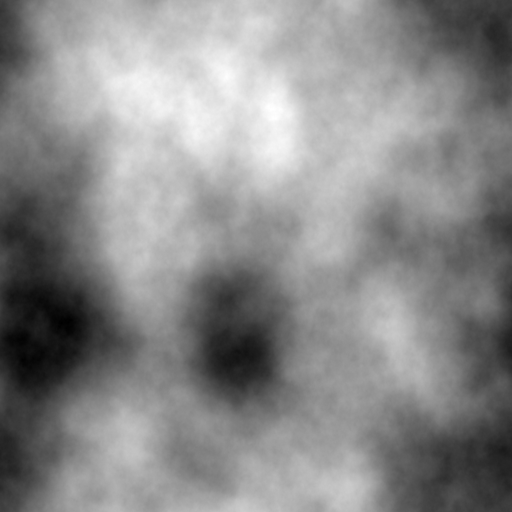
\includegraphics[scale=0.34]{figures/u_30_500km_heights.png}
 }
 \hfill
 \subtop[$\dpd{\eta(\mvec{x},t)}{x}$]
 {
 \label{sfig:derivative_x}
 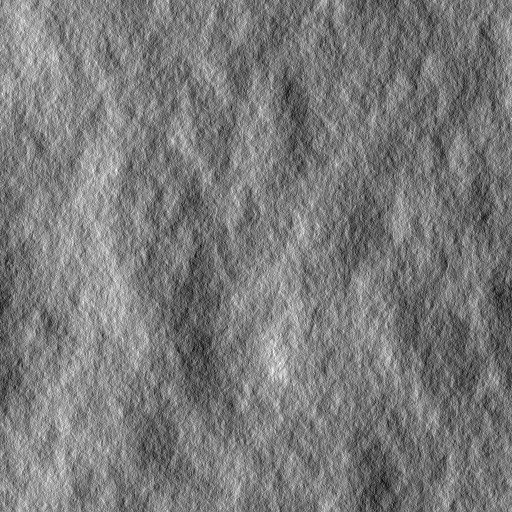
\includegraphics[scale=0.34]{figures/u_30_500km_gradient_x.png}
 }
 \hfill
 \subtop[$\dpd{\eta(\mvec{x},t)}{y}$]
 {
 \label{sfig:derivative_z}
 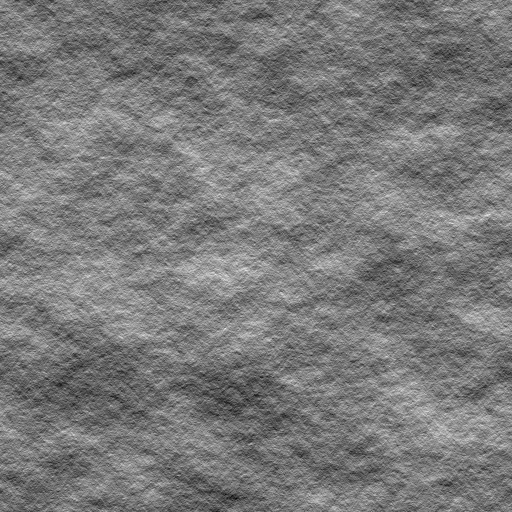
\includegraphics[scale=0.34]{figures/u_30_500km_gradient_z.png}
 }
\caption{\subcaptionref{sfig:derivative_heights} An example
surface wave height realization, displayed in greyscale (Unified spectrum, 
$U_{10}=30m\cdot s^{-1}$, $F=500km$). \subcaptionref{sfig:derivative_x} The 
X-component of the slope vector.\subcaptionref{sfig:derivative_z} The 
Y-component of the slope vector.
}
\label{fig:derivatives}
\end{figure}
%
Now we may go back to the two dimensional case, with our original two dimensional
domains $\mvec{x}$ and $\mvec{k}$. The resolution of said domains is $N \times N$,
the size of the spatial domain is $L \times L$. Let $g(\mvec{k})$ be the Discrete
Fourier Transform of $f(\mvec{x})$, then we may write the inverse Discrete Fourier
Transform in two dimensions as follows:
\begin{equation}
 f(\mvec{x}) = \sum_{\mvec{k}}g(\mvec{k})~\mathrm{e}^{\mathrm{i}\transpose{\mvec{k}}\mvec{x}}
\end{equation}
Based on Equation~\ref{eq:dft_derivative}, and by reusing Equation~\ref{eq:dft_derivative_correction}
because $N$ and $L$ are equal for both dimensions, we find the derivatives of $f(\mvec{x})$:
\begin{equation}
\label{eq:dft_derivates_2d}
 \dmd{f(\mvec{x})}{n+m}{x}{n}{y}{m} = \sum_{\mvec{k}}d(k_{x}, n)d(k_{y}, m)~g(\mvec{k})~\mathrm{e}^{\mathrm{i}\transpose{\mvec{k}}\mvec{x}}
\end{equation}
where $k_x$ and $k_y$ denote the X- and Y-component of wave vector $\mvec{k}$ 
respectively. As we need to find the surface slope vector, we need to compute 
the surface elevation's first order partial derivatives. Given surface 
elevation $\eta(\mvec{x},t)$, we obtain the two dimensional surface slope 
vector $\mvec{s}$ as follows:
\begin{equation}
\label{eq:dft_slope_2d}
 \mvec{s}(\mvec{x},t) = \left[\dpd{\eta(\mvec{x},t)}{x}, \dpd{\eta(\mvec{x},t)}{y}\right]
\end{equation}
We leave it as an exercise for the reader to substitute the terms $\eta(\mvec{x},t)$
and $h_0(\mvec{k},t)$ into Equation~\ref{eq:dft_derivates_2d} to be able to
compute the surface slope vector as given in Equation~\ref{eq:dft_slope_2d}.
Figure~\ref{fig:derivatives} depicts an example instance of surface 
elevation $\eta$ as well as its associated slopes in greyscale. Brighter 
means larger values, darker means lower values. One may notice that 
Figure~\ref{sfig:derivative_heights}, without prior knowledge, is not 
recognizable as a wave heightfield. The wave heightfield's gradients in
Figure~\ref{sfig:derivative_x} and \subcaptionref{sfig:derivative_z}, on the 
other hand, are more easily identified as water waves by the human eye.\\

The two spectra which constitute the surface slope vector in the wavevector domain
are hermitian. Therefore we are able to apply the optimisation from
Equation~\ref{eq:idft_combined} which allows us to combine both spectra into one,
obtaining both components of the surface slope vector with just one inverse Fourier transform.
%
\subsection{Normals}
%
In this work we employ a right-handed Carthesian coordinate system where the positive
Y-axis points up. The two dimensional surface slope vector $\mvec{s}$ lies in the
coordinate system's XZ-plane. Based on the surface slope vector we may find the unit
length surface normal vector $\mvec{n}$ as follows:
\begin{equation}
 \mvec{n} = \frac{(-s_x, 1, -s_y)}{\norm{(-s_x, 1, -s_y)}}
\end{equation}
where $s_x$ and $s_y$ denote the X- and Y-component of slope vector $\mvec{s}$ 
respectively.
%
\subsection{Displacements}
\label{sec:displacements}
%
\begin{figure}
 \centering
 \subtop[$\eta(\mvec{x},t)$]
 {
 \label{sfig:displacement_heights}
 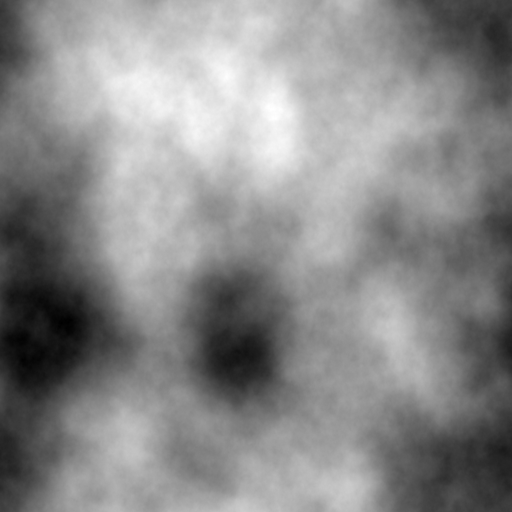
\includegraphics[scale=0.34]{figures/u_30_500km_heights.png}
 }
 \hfill
 \subtop[$D_x(\mvec{x},t)$]
 {
 \label{sfig:displacement_x}
 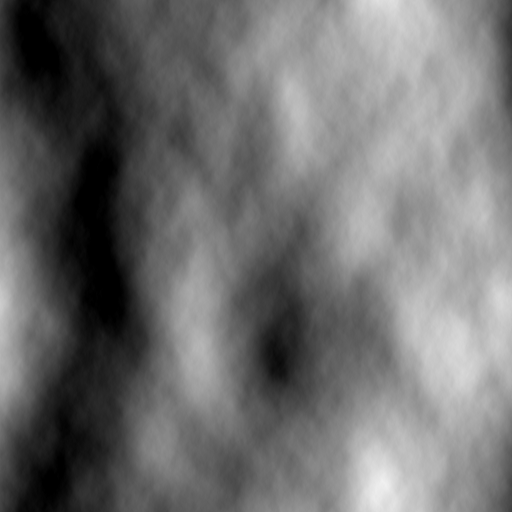
\includegraphics[scale=0.34]{figures/u_30_500km_displacement_x.png}
 }
 \hfill
 \subtop[$D_y(\mvec{x},t)$]
 {
 \label{sfig:displacement_z}
 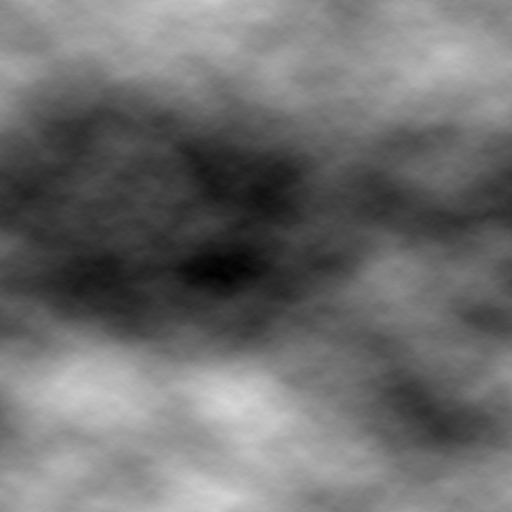
\includegraphics[scale=0.34]{figures/u_30_500km_displacement_z.png}
 }
\caption{\subcaptionref{sfig:displacement_heights}The heightfield from 
Figure~\ref{sfig:derivative_heights}.\subcaptionref{sfig:displacement_x} The 
X-component of the displacement vector.\subcaptionref{sfig:displacement_z} The 
Y-component of the displacement vector.}
\label{fig:displacements}
\end{figure}
%
The waves generated with the methods presented up to now tend to have rounded peaks and throughs,
which is typical for fair weather conditions. But we also would like to be able to synthesize waves
matching poor weather conditions, such as strong winds or even storms. During such weather, ocean waves
are sharply peaked at their tops and flattened at the bottoms. Tessendorf\cite{course:simulatingocean}
describes a Fourier Transform based method to produce such choppy waves. The concept is simple: displace
the grid points of the spatial domain in the XZ-plane, with the displacement varying locally with the waves.
Note that the displacement is a two-dimensional vector, therefore we end up computing a vector field.
Similar to spectral differentiation, we compute an inverse Fourier transform of the spectrum $h_0$
modified with an additional term. We may write the displacement vector field as follows:
\begin{align}
%\label{eq:dft_displacement}
 \mvec{D}(\mvec{x},t) &= \left[D_x(\mvec{x},t), D_y(\mvec{x},t)\right]\\
\label{eq:displacement_x} D_x(\mvec{x},t) &= \sum_{\mvec{k}}d(k_x, 
k)~h_0(\mvec{k},t)~\mathrm{e}^{\mathrm{i}\transpose{\mvec{k}}\mvec{x}} \\
\label{eq:displacement_z} D_y(\mvec{x},t) &= \sum_{\mvec{k}}d(k_y, 
k)~h_0(\mvec{k},t)~\mathrm{e}^{\mathrm{i}\transpose{\mvec{k}}\mvec{x}} \\
%\label{eq:dft_displacement_correction}
 d(l, k) &= \begin{cases}
             0 &\text{if $N$ even, and $k = 0$ or $\abs{l} = 
\frac{N}{2}\frac{2\pi}{L}$,} \\
             -\mathrm{i}\frac{l}{k} &\text{else.}
            \end{cases}
\end{align}
where the term $d(l, k)$, in addition to make sure the resulting spectrum is 
hermitian, also avoids a division by zero at $k = 0$. 
Figure~\ref{fig:displacements} shows an example instance of surface elevation 
$\eta$ as well as its associated displacements in greyscale. As before, 
brighter means larger values, darker means lower values. 
Because the spectra on the righthand side of Equations~\ref{eq:displacement_x} 
and~\ref{eq:displacement_z} are hermitian, we are again able to apply 
Equation~\ref{eq:idft_combined} and obtain both components of the displacement 
vector field with just one inverse Fourier Transform.\\

% The grid points of the spatial domain are two dimensional, $\mvec{x} = [x_x, 
% x_y]$, and lie in the XZ-plane of our three dimensional space. Embedded into 
% three dimensional space, they represent the ocean plane at rest, $\mvec{p} = 
% [x_x, 0, x_y]$. We may add surface elevation $\eta$ $[x_x, \eta(\mvec{x},t), 
% x_y]$

Given grid point $\mvec{x} = \left[ \begin{smallmatrix} x_x \\ x_y 
\end{smallmatrix}\right]$, time $t$ and surface elevation $\eta(\mvec{x},t)$, 
we may write the corresponding three dimensional, non-displaced vertex 
coordinate as follows:
\begin{equation}
 \mvec{v}(\mvec{x},t) = \begin{bmatrix}x_x\\ \eta(\mvec{x},t)\\ x_y 
\end{bmatrix} 
\end{equation}
With displacement vector $\mvec{D}(\mvec{x},t)$ at hand, according to 
Tessendorf we may compute the three dimensional, displaced vertex coordinate as 
follows:
\begin{equation}
\label{eq:displacement_gridpoints}
 \mvec{w}(\mvec{x},t) =
 \begin{bmatrix}
  x_x + u D_x(\mvec{x},t)\\ 
  \eta(\mvec{x},t)\\
  x_y + u D_y(\mvec{x},t)
 \end{bmatrix}
\end{equation}
where $u\in\mathbb{R}$ is a user-controlled parameter to scale the importance of the
displacement vector. The author of this work has found that the above formula
is correct as long as $u \leq 0$, otherwise the effect is the opposite of 
what we want to achieve. Looking at Equation~\ref{eq:displacement_gridpoints},
one can see that it is not the wave heights that are altered, but instead the grid
points on the XZ-plane are transformed based on the spatial structure of the
height field. This particular transformation accomplishes the effects we sought:
the waves' peaks are sharpened and the waves' valleys are broadened.
%
\begin{figure}
\centering
\begin{tikzpicture}
\begin{axis}[
	width=\textwidth,
	height=4cm,
    legend style={draw=none},
    %legend/.append style={nodes={right}},
	legend pos= south west,
	legend cell align=left,
	xtick = {-50, -40, -30, -20, -10, 0, 10, 20, 30, 40, 50},
	ytick = {-0.5, 0, 0.5},
    xlabel={Spatial domain coordinate~$x$~($\text{m}$)},
    ylabel={Surface height~$\eta$~($\text{m}$)},
	%enlarge y limits = 0.2,
]
\addplot[
    color=red,
    solid,
	]
    table [
		col sep=comma, 
		x expr=\thisrowno{0},
		y expr=\thisrowno{2},
	]
	{figures/u_30_500km_x_dx_h.dat};
\addlegendentry{$x$}
\addplot[
    color=blue,
    solid,
	]
    table [
		col sep=comma, 
		x expr=\thisrowno{0} - 3*\thisrowno{1},
		y expr=\thisrowno{2},
	]
	{figures/u_30_500km_x_dx_h.dat};
\addlegendentry{$x + u D_x(x,t)$}
\end{axis}
\end{tikzpicture}
\caption{Red: the original wave profile. Blue: the displaced wave profile, note 
the steep tops and the flattened valleys ($u = -3$).}
\label{fig:grid_displaced}
\end{figure}
%
Figure~\ref{fig:grid_displaced} shows two profiles of the wave height along one 
direction, where one profile uses displaced coordinates, while the other does 
not.
%
\subsection{Slopes and Displacements}
%
Based on Figure~\ref{fig:grid_displaced} it is easy to see that the application 
of displacements does not only alter the underlying grid points, but as a 
direct consequence the surface's slopes, too. Hence, we need to adjust our 
computation of the slope vector to the new circumstances. Given surface 
elevation $\eta(\mvec{x},t)$, displacement vector $\mvec{D}(\mvec{x},t)$,
and grid point transformation  $\mvec{x} + u\mvec{D}(\mvec{x},t)$, we obtain the
two dimensional surface slope
$\mvec{s}$ as follows:
\begin{equation}
\mvec{s}(\mvec{x},t) = \left[\frac{\dpd{\eta(\mvec{x},t)}{x}}{1 + u 
\dpd{D_x(\mvec{x},t)}{x}}, \frac{\dpd{\eta(\mvec{x},t)}{y}}{1 + u 
\dpd{D_y(\mvec{x},t)}{y}}\right]
\end{equation}
where $u$ is the displacement scale parameter, and $D_x$ and $D_y$ denote the X-
and Y-component of displacement vector $\mvec{D}$ respectively. Now, in addition
to surface height $\eta$, the first order partial derivatives of $\eta$, and
displacement vector $\mvec{D}$, we also need to compute a partial derivative of
$D_x$ and $D_y$ each. Again, we may compute the latter two by means of spectral
differentiation, see Equation~\ref{eq:dft_derivates_2d}. Morever, we are again
able to apply the optimisation from Equation~\ref{eq:idft_combined} which allows
us to transform the spectra of the two partial derivatives as one.
%
\subsection{Self-Intersections}
\label{sec:self_intersections}
%
\begin{figure}
\centering
\begin{tikzpicture}[
	spy using outlines={circle, magnification=5, connect spies}
]
\begin{axis}[
	width=\textwidth,
	height=4cm,
    legend style={draw=none},
    %legend/.append style={nodes={right}},
	legend pos= south west,
	legend cell align=left,
	xtick = {-50, -40, -30, -20, -10, 0, 10, 20, 30, 40, 50},
	ytick = {-0.5, 0, 0.5},
    xlabel={Spatial domain coordinate~$x$~($\text{m}$)},
    ylabel={Surface height~$\eta$~($\text{m}$)},
	axis lines = left,
	%enlarge y limits = 0.3,
]
\addplot[
    color=red!15!white,
    solid,
	forget plot
	]
    table [
		col sep=comma, 
		x expr=\thisrowno{0},
		y expr=\thisrowno{2},
	]
	{figures/u_30_500km_x_dx_h.dat};
%\addlegendentry{$x$}
\addplot[
    color=blue,
    solid,
	]
    table [
		col sep=comma, 
		x expr=\thisrowno{0} - 7.5*\thisrowno{1},
		y expr=\thisrowno{2},
	]
	{figures/u_30_500km_x_dx_h.dat};
\addlegendentry{$x + u D_x(x,t)$}
\coordinate (spypoint1) at (axis cs:-44,0.45);
\coordinate (magnifyglass1) at (axis cs:-44,2);

\coordinate (spypoint2) at (axis cs:-16,0);
\coordinate (magnifyglass2) at (axis cs:-16,2);

\coordinate (spypoint3) at (axis cs:5.5,-0.425);
\coordinate (magnifyglass3) at (axis cs:5.5,2);

\coordinate (spypoint4) at (axis cs:48.25,0.7);
\coordinate (magnifyglass4) at (axis cs:48.25,2);

\end{axis}
\spy [black, size=2cm] on (spypoint1) in node[fill=white] at (magnifyglass1);
\spy [black, size=2cm] on (spypoint2) in node[fill=white] at (magnifyglass2);
\spy [black, size=2cm] on (spypoint3) in node[fill=white] at (magnifyglass3);
\spy [black, size=2cm] on (spypoint4) in node[fill=white] at (magnifyglass4);
\end{tikzpicture}
\caption{The wave profile from Figure~\ref{fig:grid_displaced}, but with 
displacement scaling parameter $u=-7.5$ to better emphasize the effect of 
self-intersection.}
\label{fig:grid_displaced_self_intersection}
\end{figure}
%
The method by Tessendorf~\cite{course:simulatingocean} we use to generate 
choppy waves is not devoid of drawbacks. Some of the displacement vectors we 
compute may be large enough to cause the displaced geometry to self-intersect, 
see Figure~\ref{fig:grid_displaced_self_intersection}. Near the top of some 
waves the surface actually passes through itself, and as a consequence inverts, 
with the surface normal pointing inwards instead of outwards. We may get rid of 
this undesired side-effect in a rather simple way: reduce the magnitude of 
displacement scaling parameter $u$.
On the other hand, Tessendorf suggests that we use said self-intersections to 
our advantage, because they may be able to signal the breaking of waves, as 
well as the production of foam and spray. Hence, we need to be able to test
for such self-intersections in an efficient manner. Tessendorf recommends to 
compute the determinant of the~\emph{Jacobian matrix} of the transformation 
from grid point $\mvec{x}$ to displaced grid point 
$\mvec{x}+u\mvec{D}(\mvec{x},t)$. Based on the determinant we may decide if 
self-intersection is taking place.
%
%
\begin{figure}
\centering
\begin{tikzpicture}
\begin{axis}[
  width=\textwidth,
  height=10cm,
  legend style={draw=none},
  %legend/.append style={nodes={right}},
  legend pos= south west,
  legend cell align=left,
  xtick = {-50, -40, -30, -20, -10, 0, 10, 20, 30, 40, 50},
  %ytick = {-0.5, 0, 0.5},
  xlabel={Spatial domain coordinate~$x$~($\text{m}$)},
  ylabel={Surface height~$\eta$~($\text{m}$)},
  axis lines = left,
  %enlarge y limits = 0.3,
]
\addplot[
  color=ForestGreen,
  dotted,
  ]
  table [
    col sep=comma, 
    x expr=\thisrowno{0} - 7.5*\thisrowno{1},
    y expr=(1-7.5*\thisrowno{3})*(1-7.5*\thisrowno{6}) - 
    ((-7.5*\thisrowno{5}) * (-7.5*\thisrowno{4})),
  ]
  {figures/u_30_500km_x_dx_h_dxx_dxz_dzx_dzz.dat};
\addplot[
  color=red!15!white,
  solid,
  forget plot
  ]
  table [
    col sep=comma, 
    x expr=\thisrowno{0},
    y expr=\thisrowno{2},
    ]
  {figures/u_30_500km_x_dx_h_dxx_dxz_dzx_dzz.dat};
%\addlegendentry{$x$}
\addplot[
  color=blue,
  solid,
  ]
  table [
    col sep=comma, 
    x expr=\thisrowno{0} - 7.5*\thisrowno{1},
    y expr=\thisrowno{2},
    ]
  {figures/u_30_500km_x_dx_h_dxx_dxz_dzx_dzz.dat};
%\addlegendentry{$x + u D_x(x,t)$}
\addplot[
  color=black,
  solid,
  ]
  table [
    col sep=comma, 
    x expr=\thisrowno{0},
    y expr=0,
    ]
  {figures/u_30_500km_x_dx_h_dxx_dxz_dzx_dzz.dat};
%\addlegendentry{$x + u D_x(x,t)$}
\end{axis}
\end{tikzpicture}
\caption{Blue: the displaced wave profile ($u = -7.5$). Green: the Jacobian 
determinant. Note, that each instance of surface self-intersection is 
accompanied by negative Jacobian determinants.}
\label{fig:grid_displaced_j}
\end{figure}
%
First, we need the Jacobian matrix of the grid point transformation 
$\mvec{y}(\mvec{x},t)=\mvec{x}+u\mvec{D}(\mvec{x},t)$. The Jacobian matrix is 
the matrix of all first order partial derivatives of a vector valued function. 
As grid point transformation $\mvec{y}$ maps from $\mathbb{R}^2$ to 
$\mathbb{R}^2$, the Jacobian matrix is $2\times 2$ in size. Let $\mvec{J}$ be 
the Jacobian matrix of transformation $\mvec{y}$, then we may write:
%
\begin{equation}
 \label{eq:jacobian_of_displacement}
 \mvec{J}(\mvec{x},t) =
 \begin{bmatrix}
 J_{xx} & J_{xy} \\
 J_{yx} & J_{yy}
 \end{bmatrix}
 =
 \begin{bmatrix}
   1 + u\dpd{D_x(\mvec{x},t)}{x} & u\dpd{D_x(\mvec{x},t)}{y} \\
   u\dpd{D_y(\mvec{x},t)}{x} & 1 + u\dpd{D_y(\mvec{x},t)}{y}
 \end{bmatrix}
\end{equation}
where $u$ is the displacement scale parameter, and $D_x$ and $D_y$ denote the X-
and Y-component of displacement vector $\mvec{D}$ respectively.
Next, we compute the determinant of the Jacobian matrix:
\begin{equation}
 det(\mvec{J}(\mvec{x},t)) = J_{xx}J_{yy}-J_{yx}J_{xy}
\end{equation}
%
If the Jacobian determinant at $\mvec{x}$ is positive, then $\mvec{y}$ 
preserves orientation near $\mvec{x}$. If it is negative, $\mvec{y}$ reverses 
orientation. We are interested in the latter case, because wherever the 
surface self-intersects, it actually folds back on itself via a loop, and a 
loop requires a reversal of orientation. Figure~\ref{fig:grid_displaced_j} 
depicts a displaced surface, as well as the corresponding Jacobian 
determinants. One can see that wherever the surface self-intersects, the 
Jacobian determinant is negative.

% \begin{tabular}{lS[table-format = 3]S[table-format = 3.2]}
% \toprule
%   \textbf{Bus} & \multicolumn{2}{c}{\textbf{Bus Load (MVA)}} \\
%                & {Real} & {Complex} \\
%   \midrule
%   b1 &  50 &  30.99 \\
%   b2 & 170 & 105.35 \\
%   b3 & 200 & 123.94 \\
%   b4 & 150 &  49.58 \\
%   \bottomrule
% \end{tabular}

\section{Level of Detail}

The core of our ocean model are the spectra discussed in 
Section~\ref{sec:1d_frequency_spectra} and 
Section~\ref{sec:two_dimensional_frequency_spectra}. We sample the spectra in 
frequency space to obtain vertical and horizontal displacements produced by 
ocean waves. Because the sampling process is done by means of a Fourier 
Transform, the resulting data can be seamlessy tiled on the ocean surface. 
However, tiling a single perturbation pattern either leads to repetitive 
artifacts if the tile's footprint in world space is small, or to lack of detail 
if the tile's footprint in world space is large. We chose to tackle this 
issue similar to Bruneton et al.\cite{misc:oceanlightingfft} and Dupuy et 
al.\cite{article:whitecaps}, which do compute not only one perturbation 
pattern, but a set of perturbation patterns, where each pattern samples a 
different part of the spectrum. Although we are not able to remove periodicity 
from the wave field, we may increase it to the least common multiple of the
pattern periods. In practice, four different perturbation patterns suffice to
obtain satisfactory results.

In the remainder of this section we upgrade our equations to handle more than
one perturbation pattern, we explain how to parametrize the different pattern
periods to be able to sample as much of the spectrum as possible, and we discuss
the multi-resolution approach we took to reduce the computational load of pattern
data synthesis.
\subsection{Equations}
At this point, one perturbation pattern consists of surface
elevation $\eta$, displacement vector $\mvec{D}$, and the first order partial
derivatives of $\eta$, $D_x$ and $D_y$. Because we compute the surface
displacements as a sum of waves, it is straightforward to extend our
computations to incorporate not just one perturbation pattern, but a set of
patterns. Let $l \in \mathbb{N}^+$ represent the number of different patterns,
then we may compute the combined surface elevation as follows:
\begin{equation}
 z(\mvec{x},t) = \sum\limits_{i=0}^{l-1}\eta_i(\mvec{x},t)
\end{equation}
Furthermore, we may extend the horizontal grid point transformation to the
following:
\begin{equation}
\mvec{y}(\mvec{x},t) = \mvec{x}+\sum\limits_{i=0}^{l-1}u_i\mvec{D}_i(\mvec{x},t) 
\end{equation}
In lockstep with the above we compute the slope of the combined surface elevation:
\begin{equation}
\mvec{s}(\mvec{x},t) = \left[\dpd{z(\mvec{x},t)}{x},\dpd{z(\mvec{x},t)}{y}\right] = \left[\frac{\sum\limits_i \dpd{\eta_i(\mvec{x},t)}{x}}{1 
+ \sum\limits_i u_i \dpd{D_{xi}(\mvec{x},t)}{x}}, \frac{\sum\limits_i 
\dpd{\eta_i(\mvec{x},t)}{y}}{1 + \sum\limits_i 
u_i\dpd{D_{yi}(\mvec{x},t)}{y}}\right]
\end{equation}
Given the new grid point transformation, we are in need of the corresponding
Jacobian matrix to be able to locate surface self-intersections. We may write:
\begin{equation}
\label{eq:jacobian_of_displacement_multi}
 \mvec{J}(\mvec{x},t) =
 \begin{bmatrix}
 J_{xx} & J_{xy} \\
 J_{yx} & J_{yy}
 \end{bmatrix}
 =
 \begin{bmatrix}
   1 + \sum\limits_i u_i\dpd{D_{xi}(\mvec{x},t)}{x} & \sum\limits_i u_i\dpd{D_{xi}(\mvec{x},t)}{y} \\
   \sum\limits_i u_i\dpd{D_{yi}(\mvec{x},t)}{x} & 1 + \sum\limits_i u_i\dpd{D_{yi}(\mvec{x},t)}{y}
 \end{bmatrix}
\end{equation}
%
One can see that in case the number of patterns equals one, the new equations
simply fall back to the original ones.
\subsection{Sampling}
%
For us to generate a believable, as well as visually pleasing ocean surface, we
are required to include into our sum of waves a finite set of wavenumbers such
that it is representative of the whole energy. If we generate only one pattern,
based on size and resolution, we either sparsely sample inside a large
wavenumber range, or we densely sample inside a small wavenumber range. The
former results in a poor reconstruction of a larger part of the spectrum, the
latter in a better reconstruction of a smaller part of the spectrum, but
possibly missing other relevant parts of the spectrum. Thus, we generate more
than one pattern, where the goal is for each pattern to sample as many distinct
wavenumbers as possible.
%
\begin{figure}
\centering
\begin{tikzpicture}
\begin{groupplot}[
	group style={
		columns=4,
		rows=1,
		xlabels at=edge bottom,
		ylabels at=edge left,
	},
    xlabel={$k_d$},
    ylabel=\empty,
	width=0.3\textwidth,
	axis x line=bottom,
%	ymin = 0,
%	ymax = 0.001,
	]
\nextgroupplot[
	ytick=\empty,
	axis y line=none,
	title = {(a) $L=100m$},
	xmin = 0,
	xmax = 1.4,
	]
\addplot[
  color=red,
  %mark color=blue,
  %mark=halfdiamond*,
  fill,
  fill opacity=0.2,
  ]
  table [
    col sep=comma, 
  ]
  {figures/sampling_res_12_area_100.dat} \closedcycle;
\addplot[
  ycomb,
  color=red,
  ]
  table [
    col sep=comma, 
  ]
  {figures/sampling_res_12_area_100.dat};
\nextgroupplot[
	ytick=\empty,
	axis y line=none,
	title = {(b) $L=50m$},
	xmin = 0,
	xmax = 1.4,
	]
\addplot[
  color=red,
  fill,
  fill opacity=0.2,
  ]
  table [
    col sep=comma, 
  ]
  {figures/sampling_res_12_area_50.dat} \closedcycle;
\addplot[
  ycomb,
  color=red,
  ]
  table [
    col sep=comma, 
  ]
  {figures/sampling_res_12_area_50.dat};
\nextgroupplot[
	ytick=\empty,
	axis y line=none,
	title = {(c) $N=12$},
	xmin = 0,
	xmax = 1.5,
	]
\addplot[
  color=blue,
  fill,
  fill opacity=0.2,
  ]
  table [
    col sep=comma, 
  ]
  {figures/sampling_area_100_res_12.dat} \closedcycle;
\addplot[
  ycomb,
  color=blue,
  ]
  table [
    col sep=comma, 
  ]
  {figures/sampling_area_100_res_12.dat};
\nextgroupplot[
	ytick=\empty,
	axis y line=none,
	title = {(d) $N=24$},
	xmin = 0,
	xmax = 1.5,
	]
\addplot[
  color=blue,
  fill,
  fill opacity=0.2,
  ]
  table [
    col sep=comma, 
  ]
  {figures/sampling_area_100_res_24.dat} \closedcycle;
\addplot[
  ycomb,
  color=blue,
  ]
  table [
    col sep=comma, 
  ]
  {figures/sampling_area_100_res_24.dat};
\end{groupplot}
\end{tikzpicture}
\caption{Red: Equal resolution, different size $L$. Both, (a) and (b), consist
of the same number of samples, $N=12$. (a) covers a smaller wavenumber range
than (b) because the former employs a smaller distance between consecutive
sample points.
Blue: Equal size, $L=100m$, different resolution $N$. The distance between
consecutive sample points is equivalent in (c) and (d). (d) covers a larger
wavenumber range because it contains more samples than (c).}
\label{fig:sampling_area_vs_res}
\end{figure}
%

Recall that both, the spatial domain and the wavevector domain, are defined
entirely by size $L$ and resolution $N$. The smallest wavenumber
$k = \norm{\mvec{k}}$, where $k > 0$, representable by the wavevector domain is
$k = 2\pi/L$, it depends only on size. Moreover, the distance between subsequent
sample points in both dimensions, $\Delta k$, is defined as $\Delta k = 2\pi/L$.
Hence, $\Delta k$ depends only on size. Therefore, by choosing size $L$, we do
not only define the minimal wavenumber we are able to sample, but also define
how densely we are able to sample the spectrum. The largest wavenumber contained
in the wavevector domain is $k = \sqrt{2}\pi N/L$. So, given size $L$,
resolution $N$ defines how large the wavenumbers are allowed to grow, giving us
an upper limit of the wavenumbers involved in the sum of waves. In short, with
size $L$ and resolution $N$ specified for a pattern, we are able to compute the
pattern's wavenumber range.

Let $k_d$ be a set of distinct wavenumbers based on parameters $L$ and $N$. With
the wavenumber set $k_d$ at hand we may sample a one-dimensional wavenumber
spectrum. Figure~\ref{fig:sampling_area_vs_res} depicts a set of reconstructions
of one specific one-dimensional wavenumber spectrum, where one can see the
effects of size $L$ and resolution $N$ on the wavenumber set $k_d$, and thus on
the reconstructed pattern.

With size $L$ and resolution $N$ specified for a pattern, we may compute the
pattern's wavenumber range. Since we would like to sample the spectrum at as
many wavenumbers as possible, we need to minimize overlap of the wavenumber
ranges of different patterns. Our implementation employs the same resolution for
all patterns, therefore we focus on pattern
size to reduce wavenumber overlap. We need at least one large pattern size, to
avoid repetitive artifacts as much as possible, and one small pattern size for
closeup detail. In addition, we have to look out for the different sizes not to
be integral multiples of each other, otherwise the surface may seem repetitive
at a smaller scale than expected. We chose to tackle both requirements by
employing multiples based on the golden ratio $\varphi = (1 + \sqrt{5})/2$. The
user sets the largest desired pattern size, each following pattern size is
reduced by the same multiplicative factor $f$, where $f \in \{\varphi^{-1},
1 - \varphi^{-1}\}$.
%
\begin{figure}
\centering
\begin{tikzpicture}
\begin{groupplot}[
	group style={
		columns=4,
		rows=2,
		%xlabels at=edge bottom,
		xlabels at=all,
		ylabels at=edge left,
	},
    xlabel={$k$},
    ylabel=\empty,
	width=0.3\textwidth,
	axis x line=bottom,
%	ymin = 0,
%	ymax = 0.001,
	]
\nextgroupplot[
	ytick=\empty,
	axis y line=none,
	]
\addplot[
  color=red,
  fill,
  fill opacity=0.2,
  unbounded coords=discard,
  ]
  table [
    col sep=comma, 
  ]
  {figures/sampling_scale_03_lod_1.dat} \closedcycle;
\nextgroupplot[
	ytick=\empty,
	axis y line=none,
	]
\addplot[
  color=blue,
  fill,
  fill opacity=0.2,
  unbounded coords=discard,
  ]
  table [
    col sep=comma, 
  ]
  {figures/sampling_scale_03_lod_2.dat} \closedcycle;
\nextgroupplot[
	ytick=\empty,
	axis y line=none,
	]
\addplot[
  color=green,
  fill,
  fill opacity=0.2,
  unbounded coords=discard,
  ]
  table [
    col sep=comma, 
  ]
  {figures/sampling_scale_03_lod_3.dat} \closedcycle;
\nextgroupplot[
	ytick=\empty,
	axis y line=none,
	]
\addplot[
  color=yellow,
  fill,
  fill opacity=0.2,
  unbounded coords=discard,
  ]
  table [
    col sep=comma, 
  ]
  {figures/sampling_scale_03_lod_4.dat} \closedcycle;
\nextgroupplot[
	ytick=\empty,
	axis y line=none,
	]
\addplot[
  color=red,
  fill,
  fill opacity=0.2,
  unbounded coords=discard,
  ]
  table [
    col sep=comma, 
  ]
  {figures/sampling_scale_06_lod_1.dat} \closedcycle;
\nextgroupplot[
	ytick=\empty,
	axis y line=none,
	]
\addplot[
  color=blue,
  fill,
  fill opacity=0.2,
  unbounded coords=discard,
  ]
  table [
    col sep=comma, 
  ]
  {figures/sampling_scale_06_lod_2.dat} \closedcycle;
\nextgroupplot[
	ytick=\empty,
	axis y line=none,
	]
\addplot[
  color=green,
  fill,
  fill opacity=0.2,
  unbounded coords=discard,
  ]
  table [
    col sep=comma, 
  ]
  {figures/sampling_scale_06_lod_3.dat} \closedcycle;
\nextgroupplot[
	ytick=\empty,
	axis y line=none,
	]
\addplot[
  color=yellow,
  fill,
  fill opacity=0.2,
  unbounded coords=discard,
  ]
  table [
    col sep=comma, 
  ]
  {figures/sampling_scale_06_lod_4.dat} \closedcycle;
\end{groupplot}
\end{tikzpicture}
\caption{Top row: reconstructed spectra of patterns with sizes reduced by
 $1-\varphi^{-1}$. Bottom row: reconstructed spectra of patterns with sizes
reduced by $\varphi^{-1}$.}
\label{fig:sampling_pattern_size_reduction}
\end{figure}
%

In case we choose $f = 1-\varphi^{-1} \approx 0.382$, the combined patterns
allow for tight sampling around the spectral peak as well as in the high
wavenumber range. Hence, the sum of waves includes both, large wavelengths which
give the overall surface its shape, and small wavelengths for close-up detail.
The drawback of this choice are the smaller pattern sizes, which results in
repetitive artifacts at a smaller scale than expected. In case we choose
$f = \varphi^{-1} \approx 0.618$, the combined patterns allow for even more
tight sampling around the spectral peak, but missing most of the energy in the
high wavenumber range. Thus, it is the large wavelengths we are able to
reconstruct, but missing close-up detail. On the other hand, we have less issues
with repetitve artifacts. The two rows in Figure~\ref{fig:sampling_pattern_size_reduction}
depict the reconstructions of one and the same spectrum, based on patterns with
the same resolution $N$, but initial size $L$ reduced by the two different
factors.

%
%
\begin{figure}
\centering
\begin{tikzpicture}
\begin{groupplot}[
	group style={
		columns=3,
		rows=2,
		%xlabels at=edge bottom,
		xlabels at=all,
		ylabels at=edge left,
	},
    xlabel={$k$},
    ylabel=\empty,
	width=0.35\textwidth,
	axis x line=bottom,
%	ymin = 0,
%	ymax = 0.001,
	]
\nextgroupplot[
	ytick=\empty,
	axis y line=none,
	]
\addplot[
  color=red,
  fill,
  fill opacity=0.2,
  ]
  table [
    col sep=comma, 
  ]
  {figures/sampling_scale_03_lod_1.dat} \closedcycle;
\addplot[
  color=blue,
  fill,
  fill opacity=0.2,
  ]
  table [
    col sep=comma, 
  ]
  {figures/sampling_scale_03_lod_2_capped.dat} \closedcycle;
\nextgroupplot[
	ytick=\empty,
	axis y line=none,
	]
\addplot[
  color=red,
  fill,
  fill opacity=0.2,
  ]
  table [
    col sep=comma, 
  ]
  {figures/sampling_scale_03_lod_1.dat} \closedcycle;
\addplot[
  color=blue,
  fill,
  fill opacity=0.2,
  ]
  table [
    col sep=comma, 
  ]
  {figures/sampling_scale_03_lod_2_capped.dat} \closedcycle;
\addplot[
  color=green,
  fill,
  fill opacity=0.2,
  ]
  table [
    col sep=comma, 
  ]
  {figures/sampling_scale_03_lod_3_capped.dat} \closedcycle;
\nextgroupplot[
	ytick=\empty,
	axis y line=none,
	]
\addplot[
  color=red,
  fill,
  fill opacity=0.2,
  ]
  table [
    col sep=comma, 
  ]
  {figures/sampling_scale_03_lod_1.dat} \closedcycle;
\addplot[
  color=blue,
  fill,
  fill opacity=0.2,
  ]
  table [
    col sep=comma, 
  ]
  {figures/sampling_scale_03_lod_2_capped.dat} \closedcycle;
\addplot[
  color=green,
  fill,
  fill opacity=0.2,
  ]
  table [
    col sep=comma, 
  ]
  {figures/sampling_scale_03_lod_3_capped.dat} \closedcycle;
\addplot[
  color=yellow,
  fill,
  fill opacity=0.2,
  ]
  table [
    col sep=comma, 
  ]
  {figures/sampling_scale_03_lod_4_capped.dat} \closedcycle;
\nextgroupplot[
	ytick=\empty,
	axis y line=none,
	]
\addplot[
  color=red,
  fill,
  fill opacity=0.2,
  ]
  table [
    col sep=comma, 
  ]
  {figures/sampling_scale_06_lod_1.dat} \closedcycle;
\addplot[
  color=blue,
  fill,
  fill opacity=0.2,
  ]
  table [
    col sep=comma, 
  ]
  {figures/sampling_scale_06_lod_2_capped.dat} \closedcycle;
\nextgroupplot[
	ytick=\empty,
	axis y line=none,
	]
\addplot[
  color=red,
  fill,
  fill opacity=0.2,
  ]
  table [
    col sep=comma, 
  ]
  {figures/sampling_scale_06_lod_1.dat} \closedcycle;
\addplot[
  color=blue,
  fill,
  fill opacity=0.2,
  ]
  table [
    col sep=comma, 
  ]
  {figures/sampling_scale_06_lod_2_capped.dat} \closedcycle;
\addplot[
  color=green,
  fill,
  fill opacity=0.2,
  ]
  table [
    col sep=comma, 
  ]
  {figures/sampling_scale_06_lod_3_capped.dat} \closedcycle;
\nextgroupplot[
	ytick=\empty,
	axis y line=none,
	]
\addplot[
  color=red,
  fill,
  fill opacity=0.2,
  ]
  table [
    col sep=comma, 
  ]
  {figures/sampling_scale_06_lod_1.dat} \closedcycle;
\addplot[
  color=blue,
  fill,
  fill opacity=0.2,
  ]
  table [
    col sep=comma, 
  ]
  {figures/sampling_scale_06_lod_2_capped.dat} \closedcycle;
\addplot[
  color=green,
  fill,
  fill opacity=0.2,
  ]
  table [
    col sep=comma, 
  ]
  {figures/sampling_scale_06_lod_3_capped.dat} \closedcycle;
\addplot[
  color=yellow,
  fill,
  fill opacity=0.2,
  ]
  table [
    col sep=comma, 
  ]
  {figures/sampling_scale_06_lod_4_capped.dat} \closedcycle;
\end{groupplot}
\end{tikzpicture}
\caption{Gradual assembly of the reconstructed spectra from Figure
\ref{fig:sampling_pattern_size_reduction}.}
\label{fig:sampling_pattern_assembly}
\end{figure}
%
Care has to be taken not to sample the same part of the spectrum multiple times.
Not doing so, would imply including the same wavenumber(s) multiple times in the
sum of waves. Thus, if the spectrum of one pattern already covers a specific
wavenumber range, a second spectrum covering parts or the entirety of that same
range, has to be zeroed in the region of overlap.
Figure~\ref{fig:sampling_pattern_assembly} shows the assembly of the overlapping
spectra from Figure~\ref{fig:sampling_pattern_size_reduction} into one coherent
spectrum. The transition from data from one spectrum to data from the next
spectrum always happens at the maximum wavenumber of the spectrum with the
smaller wavenumber range.

\emph{Note}: The typical profile of a one dimensional wavenumber spectrum suggests
that it would be beneficial to employ an adaptive sampling scheme which allows
for tight sampling in the low wavenumber range, especially near the peak
wavenumber, and sparse sampling in the high wavenumber range, see
Fr\'{e}chot~\cite{article:frechot2007}. Because we employ a Discrete Fourier
Transform to compute the sum of waves, we are subject to its constraints. One of
those constraints is that the spacing between subsequent coordinates is constant,
namely $\Delta k$. Hence, in combination with a Discrete Fourier Transform, we
are not allowed to employ a sampling scheme where $\Delta k$ changes dependent
on which part of the wavenumber profile is being sampled.


\subsection{Resolutions}
%
%
\begin{figure}
\centering
\begin{tikzpicture}
\begin{groupplot}[
	group style={
		columns=4,
		rows=2,
		%xlabels at=edge bottom,
		xlabels at=all,
		ylabels at=edge left,
	},
    xlabel={$k$},
    ylabel=\empty,
	width=0.3\textwidth,
	axis x line=bottom,
%	ymin = 0,
%	ymax = 0.001,
	]
\nextgroupplot[
	ytick=\empty,
	axis y line=none,
	xmin = 0,
	xmax = 0.46,
	]
\addplot[
  color=red!20!white,
  ]
  table [
    col sep=comma, 
  ]
  {figures/sampling_multires_scale_06_res_128_8_lod_1.dat};
\addplot[
  color=red,
  %draw=red,
  fill,
  fill opacity=0.2,
  ]
  table [
    col sep=comma, 
  ]
  {figures/sampling_multires_scale_06_res_64_8_lod_1.dat} \closedcycle;
\addplot[
  ycomb,
  color=red,
  ]
  table [
    col sep=comma, 
  ]
  {figures/sampling_multires_scale_06_res_64_8_lod_1.dat};
\nextgroupplot[
	ytick=\empty,
	axis y line=none,
	xmin = 0,
	xmax = 0.74,
	]
\addplot[
  color=blue!20!white,
  ]
  table [
    col sep=comma, 
  ]
  {figures/sampling_multires_scale_06_res_128_8_lod_2.dat};
\addplot[
  ycomb,
  color=blue,
  ]
  table [
    col sep=comma, 
  ]
  {figures/sampling_multires_scale_06_res_64_8_lod_2.dat};
\addplot[
  color=blue,
  fill,
  fill opacity=0.2,
  ]
  table [
    col sep=comma, 
  ]
  {figures/sampling_multires_scale_06_res_64_8_lod_2.dat} \closedcycle;
\nextgroupplot[
	ytick=\empty,
	axis y line=none,
	xmin = 0,
	xmax = 1.2,
	]
\addplot[
  color=green!20!white,
  ]
  table [
    col sep=comma, 
  ]
  {figures/sampling_multires_scale_06_res_128_8_lod_3.dat};
\addplot[
  ycomb,
  color=green,
  ]
  table [
    col sep=comma, 
  ]
  {figures/sampling_multires_scale_06_res_64_8_lod_3.dat};
\addplot[
  color=green,
  fill,
  fill opacity=0.2,
  ]
  table [
    col sep=comma, 
  ]
  {figures/sampling_multires_scale_06_res_64_8_lod_3.dat} \closedcycle;
\nextgroupplot[
	ytick=\empty,
	axis y line=none,
	xmin = 0,
	xmax = 1.94,
	]
\addplot[
  color=yellow!20!white,
  ]
  table [
    col sep=comma, 
  ]
  {figures/sampling_multires_scale_06_res_128_8_lod_4.dat};
\addplot[
  ycomb,
  color=yellow,
  ]
  table [
    col sep=comma, 
  ]
  {figures/sampling_multires_scale_06_res_64_8_lod_4.dat};
\addplot[
  color=yellow,
  fill,
  fill opacity=0.2,
  ]
  table [
    col sep=comma, 
  ]
  {figures/sampling_multires_scale_06_res_64_8_lod_4.dat} \closedcycle;
\nextgroupplot[
	ytick=\empty,
	axis y line=none,
	xmin = 0,
	xmax = 0.46,
	]
\addplot[
  color=red,
  fill,
  fill opacity=0.2,
  ]
  table [
    col sep=comma, 
  ]
  {figures/sampling_multires_scale_06_res_128_8_lod_1.dat} \closedcycle;
\addplot[
  ycomb,
  color=red,
  ]
  table [
    col sep=comma, 
  ]
  {figures/sampling_multires_scale_06_res_128_8_lod_1.dat};
\nextgroupplot[
	ytick=\empty,
	axis y line=none,
	xmin = 0,
	xmax = 0.74,
	]
\addplot[
  color=blue,
  fill,
  fill opacity=0.2,
  ]
  table [
    col sep=comma, 
  ]
  {figures/sampling_multires_scale_06_res_128_8_lod_2.dat} \closedcycle;
\addplot[
  ycomb,
  color=blue,
  ]
  table [
    col sep=comma, 
  ]
  {figures/sampling_multires_scale_06_res_128_8_lod_2.dat};
\nextgroupplot[
	ytick=\empty,
	axis y line=none,
	xmin = 0,
	xmax = 1.2,
	]
\addplot[
  color=green,
  fill,
  fill opacity=0.2,
  ]
  table [
    col sep=comma, 
  ]
  {figures/sampling_multires_scale_06_res_128_8_lod_3.dat} \closedcycle;
\addplot[
  ycomb,
  color=green,
  ]
  table [
    col sep=comma, 
  ]
  {figures/sampling_multires_scale_06_res_128_8_lod_3.dat};
\nextgroupplot[
	ytick=\empty,
	axis y line=none,
	xmin = 0,
	xmax = 1.94,
	]
\addplot[
  color=yellow,
  fill,
  fill opacity=0.2,
  ]
  table [
    col sep=comma, 
  ]
  {figures/sampling_multires_scale_06_res_128_8_lod_4.dat} \closedcycle;
\addplot[
  ycomb,
  color=yellow,
  ]
  table [
    col sep=comma, 
  ]
  {figures/sampling_multires_scale_06_res_128_8_lod_4.dat};
\end{groupplot}
\end{tikzpicture}
\caption{Reconstructions of one and the same spectrum. Top and bottom row use
equal pattern sizes, it follows that both rows have matching distances between
subsequent samples. Top row employs half the resolution of bottom row, therefore
each of its reconstructions is equal the left half of the correspondig
reconstruction in bottom row.}
\label{fig:sampling_different_resolutions}
\end{figure}
%
%
Recall, that one perturbation pattern consists of surface elevation $\eta$,
displacement vector $\mvec{D}$, and the first order partial derivatives of
$\eta$ and $\mvec{D}$. Moreover, we have a set of such patterns. The
computational load to synthesize all the cumulated pattern data has proven to be
substantial. To improve upon the status quo, we chose to implement an approach
common in computer graphics: augment low resolution geometry with high resolution
surface information to generate detailed lighting. For our specific case, that
means we may synthesize vertical and horizontal displacements at a lower
resolution than the associated first order partial derivatives.
%
%
Given pattern size $L$, grid point spacing $\Delta k = 2\pi/L$, pattern
resolutions $N_h,N_l \in \mathbb{N}$ with $N_l < N_h$, then we may define the
two following wavevector domains:
%
\begin{align}
\mvec{h} = (k_x,k_y)~&\in~\{(\alpha\Delta k,\alpha\Delta k)|-\frac{N_h}{2}\leq\alpha<\frac{N_h}{2}\}\\
\mvec{l} = (k_x,k_y)~&\in~\{(\alpha\Delta k,\alpha\Delta k)|-\frac{N_l}{2}\leq\alpha<\frac{N_l}{2}\}
\end{align}
where $\mvec{h}$ is based on the higher resolution $N_h$ and therefore contains
more pairs $(k_x, k_y)$ than $\mvec{l}$. One may notice that $\mvec{l}$ is a
subset of $\mvec{h}$, all pairs $(k_x, k_y)$ in $\mvec{l}$ are also to be found
in $\mvec{h}$. Hence, there is no need to generate two separate instances of the
wave energy spectrum with differing resolutions.
As long as the two different wavevector domains are based on
the same pattern size, $\mvec{l}$ is a subset of $\mvec{h}$, it follows that
$\Theta(\mvec{l})$ is a subset of $\Theta(\mvec{h})$. In short, the low
resolution variant of the wave energy spectrum is already embedded inside the
high resolution variant. See Figure~\ref{fig:sampling_different_resolutions} for
a display of the relation between two reconstructions of the same one
dimensional wavenumber spectrum with different resolutions, but the same size.
%
%
\begin{figure}
\centering
\begin{tikzpicture}
\begin{groupplot}[
	group style={
		columns=3,
		rows=2,
		%xlabels at=edge bottom,
		xlabels at=all,
		ylabels at=edge left,
	},
    xlabel={$k$},
    ylabel=\empty,
	width=0.375\textwidth,
	axis x line=bottom,
%	ymin = 0,
%	ymax = 0.001,
	]
\nextgroupplot[
	ytick=\empty,
	axis y line=none,
	]
\addplot[
  color=red,
  fill,
  fill opacity=0.2,
  ]
  table [
    col sep=comma, 
  ]
  {figures/sampling_multires_scale_06_res_64_8_lod_1_capped.dat} \closedcycle;
\addplot[
  color=blue,
  fill,
  fill opacity=0.2,
  ]
  table [
    col sep=comma, 
  ]
  {figures/sampling_multires_scale_06_res_64_8_lod_2_capped.dat} \closedcycle;
\nextgroupplot[
	ytick=\empty,
	axis y line=none,
	]
\addplot[
  color=red,
  fill,
  fill opacity=0.2,
  ]
  table [
    col sep=comma, 
  ]
  {figures/sampling_multires_scale_06_res_64_8_lod_1_capped.dat} \closedcycle;
\addplot[
  color=blue,
  fill,
  fill opacity=0.2,
  ]
  table [
    col sep=comma, 
  ]
  {figures/sampling_multires_scale_06_res_64_8_lod_2_capped.dat} \closedcycle;
\addplot[
  color=green,
  fill,
  fill opacity=0.2,
  ]
  table [
    col sep=comma, 
  ]
  {figures/sampling_multires_scale_06_res_64_8_lod_3_capped.dat} \closedcycle;
\nextgroupplot[
	ytick=\empty,
	axis y line=none,
	]
\addplot[
  color=red,
  fill,
  fill opacity=0.2,
  ]
  table [
    col sep=comma, 
  ]
  {figures/sampling_multires_scale_06_res_64_8_lod_1_capped.dat} \closedcycle;
\addplot[
  color=blue,
  fill,
  fill opacity=0.2,
  ]
  table [
    col sep=comma, 
  ]
  {figures/sampling_multires_scale_06_res_64_8_lod_2_capped.dat} \closedcycle;
\addplot[
  color=green,
  fill,
  fill opacity=0.2,
  ]
  table [
    col sep=comma, 
  ]
  {figures/sampling_multires_scale_06_res_64_8_lod_3_capped.dat} \closedcycle;
\addplot[
  color=yellow,
  fill,
  fill opacity=0.2,
  ]
  table [
    col sep=comma, 
  ]
  {figures/sampling_multires_scale_06_res_64_8_lod_4_capped.dat} \closedcycle;
\nextgroupplot[
	ytick=\empty,
	axis y line=none,
	]
\addplot[
  color=red,
  fill,
  fill opacity=0.2,
  ]
  table [
    col sep=comma, 
  ]
  {figures/sampling_multires_scale_06_res_128_8_lod_1_capped.dat} \closedcycle;
\addplot[
  color=blue,
  fill,
  fill opacity=0.2,
  ]
  table [
    col sep=comma, 
  ]
  {figures/sampling_multires_scale_06_res_128_8_lod_2_capped.dat} \closedcycle;
\nextgroupplot[
	ytick=\empty,
	axis y line=none,
	]
\addplot[
  color=red,
  fill,
  fill opacity=0.2,
  ]
  table [
    col sep=comma, 
  ]
  {figures/sampling_multires_scale_06_res_128_8_lod_1_capped.dat} \closedcycle;
\addplot[
  color=blue,
  fill,
  fill opacity=0.2,
  ]
  table [
    col sep=comma, 
  ]
  {figures/sampling_multires_scale_06_res_128_8_lod_2_capped.dat} \closedcycle;
\addplot[
  color=green,
  fill,
  fill opacity=0.2,
  ]
  table [
    col sep=comma, 
  ]
  {figures/sampling_multires_scale_06_res_128_8_lod_3_capped.dat} \closedcycle;
\nextgroupplot[
	ytick=\empty,
	axis y line=none,
	]
\addplot[
  color=red,
  fill,
  fill opacity=0.2,
  ]
  table [
    col sep=comma, 
  ]
  {figures/sampling_multires_scale_06_res_128_8_lod_1_capped.dat} \closedcycle;
\addplot[
  color=blue,
  fill,
  fill opacity=0.2,
  ]
  table [
    col sep=comma, 
  ]
  {figures/sampling_multires_scale_06_res_128_8_lod_2_capped.dat} \closedcycle;
\addplot[
  color=green,
  fill,
  fill opacity=0.2,
  ]
  table [
    col sep=comma, 
  ]
  {figures/sampling_multires_scale_06_res_128_8_lod_3_capped.dat} \closedcycle;
\addplot[
  color=yellow,
  fill,
  fill opacity=0.2,
  ]
  table [
    col sep=comma, 
  ]
  {figures/sampling_multires_scale_06_res_128_8_lod_4_capped.dat} \closedcycle;
\end{groupplot}
\end{tikzpicture}
\caption{Gradual assembly of the reconstructed spectra from Figure
\ref{fig:sampling_different_resolutions}. Top row and bottom row transition
between two subsequent reconstructions at different wavenumbers.}
\label{fig:sampling_different_resolutions_pattern_assembly}
\end{figure}
%
%

At this point we have two sets of reconstructions of the same spectrum, based on
two different resolutions. For each set, we need to assemble the overlapping
spectral data into one coherent spectrum. As before, the transition from one
reconstruction to the next takes place at the maximum wavenumber of the
reconstruction with the smaller wavenumber range. In addition, we must take
into consideration that the two sets of spectral data have different wavenumber
ranges, therefore the transitions may take place at different wavenumbers. Figure
\ref{fig:sampling_different_resolutions_pattern_assembly} depicts the gradual
assembly of the spectral data from Figure
\ref{fig:sampling_different_resolutions}.\\

Recall Equation~\ref{eq:dft_surface_elevation}, where we synthesize a random
surface based on wavevector domain $\mvec{k}$. For each wavevector we compute
wave energy $\Theta(\mvec{k})$ and generate a pair of standard normal
distributed random numbers $(\xi_r,\xi_i)$. Now, if we would like to generate
an instance of the same surface at a lower resolution, we need to take the
following steps:
\begin{itemize}
 \item Define a wavevector domain $\mvec{l}$ with a lower resolution than
 wavevector domain $\mvec{k}$, but the same underlying size $L$.
 \item Extract subset $\Theta(\mvec{l})$ from $\Theta(\mvec{k})$.
 \item For each extracted element of $\Theta(\mvec{k})$, also copy its
 associated random number pair $(\xi_r,\xi_i)$.
\end{itemize}
The last step makes sure that each wavevector is associated with one specific
pair of random numbers, be it as part of the low resolution surface as well as
part of the high resolution surface. The random number pair basically defines
the amplitude associated with a wavevector. To be able to reproduce the same
random surface at different resolutions, the pairing between amplitude and
wavevector needs to remain the same across resolutions.

\section{Demo Application}
For showcasing purposes we implemented a compact demo application on Linux.
It is written in Objective-C and employs the GNUstep\cite{misc:gnustep}
Base Library which provides container classes as well as basic algorithms.
We use the compatibility profile of OpenGL\cite{misc:opengl} version 3.3
\cite{misc:opengl33} for rendering, where the GLFW library\cite{misc:glfw}
handles the creation of a window with the desired OpenGL context. Moreover,
it is GLFW which gives us the means to handle mouse and keyboard input.
All of the ocean energy spectra presented in this work were, in a first step,
implemented in MATLAB\cite{misc:matlab}. This allowed for easy analysis,
debugging and visualisation. Only in a second step did we integrate the energy
spectra into the demo application, making sure the results match the ones of
the MATLAB version. In addition, we chose to employ the same library for
Fast Fourier Transforms as MATLAB, namely FFTW\cite{misc:fftw}. FFTW does
not only provide a standard complex-to-complex DFT, but also a more specialised
complex-to-real DFT, which proves to be beneficial for our use case.

The application consists of three running threads: the first thread continuously
generates frequency spectra for the desired number of patterns, then hands them
to a second thread which applies the inverse DFT on said spectra. The transformed
data is then given to the main thread for rendering.

The user is given a wide range of control over frequency spectrum generation.
He may configure the number of patterns, the resolution of the vertical and horizontal
displacements, the resolution of the first order partial derivatives,
the spectrum type, wind velocity $U_{10}$, the size $L$ of the largest pattern,
and fetch $F$.


Preetham Sky + Sun Disc\cite{Preetham:1999}
Bruneton Seamless Ocean Lighting \cite{article:oceanlighting}\cite{misc:oceanlightingfft}
Ocean Whitecaps\cite{article:whitecaps}

\subsubsection{Projected Grid}
Projected Grid\cite{thesis:johanson}
\subsubsection{Skylight}
%
\begin{figure}
 \centering
 \subtop[Sky]
 {
 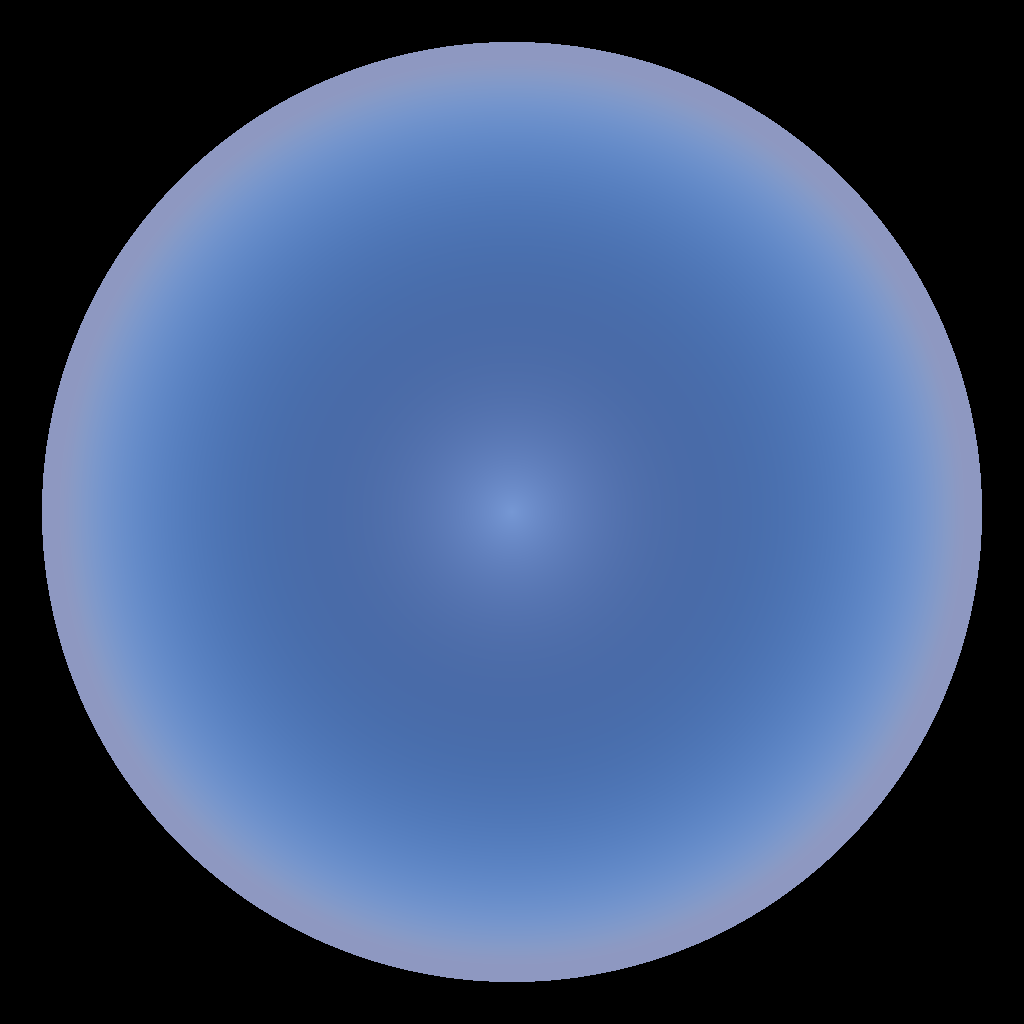
\includegraphics[scale=0.125]{figures/preetham_1.png}
 }
 \subtop[Sky + Solar Disc]
 {
 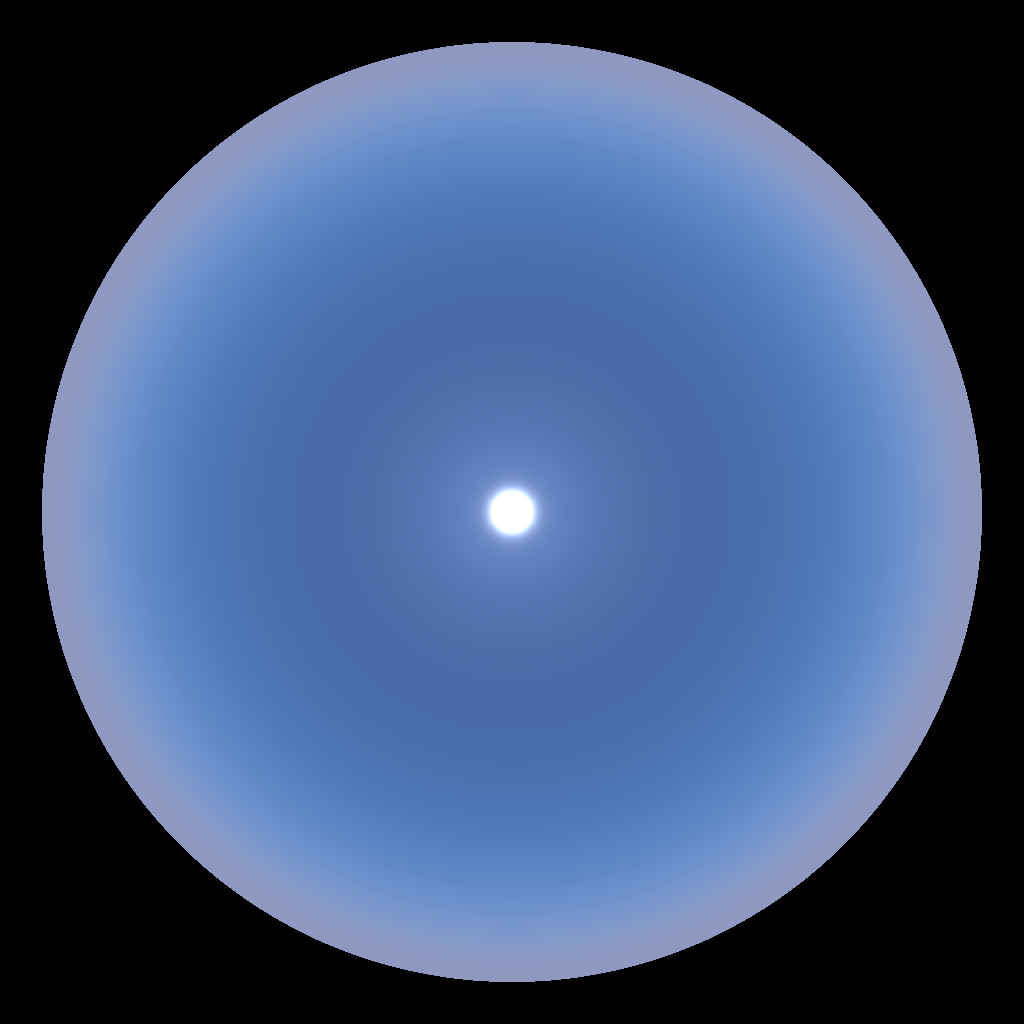
\includegraphics[scale=0.125]{figures/preetham_solar_disk_1.png}
 }
 \subtop[Sky + Solar Disc + Irradiance]
 {
 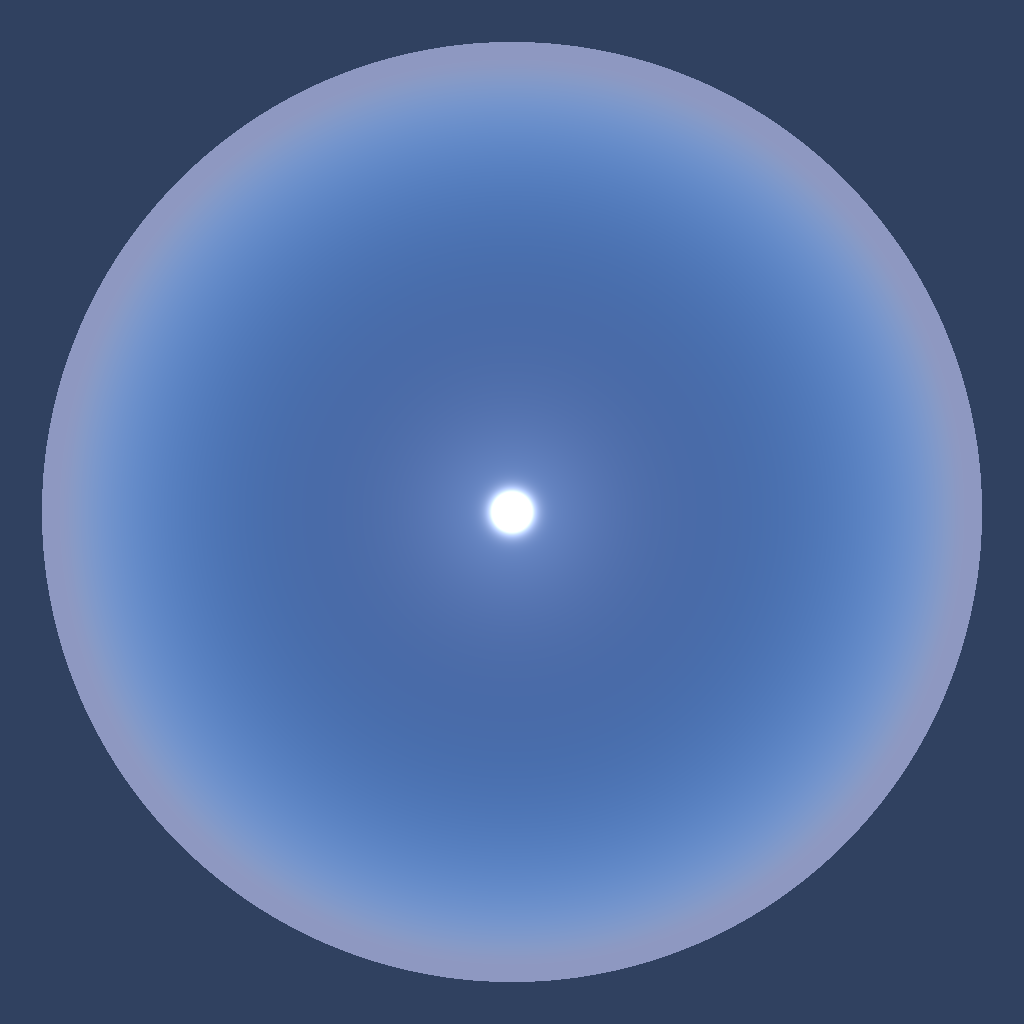
\includegraphics[scale=0.125]{figures/preetham_solar_disk_irradiance_1.png}
 }
 \subtop
 {
 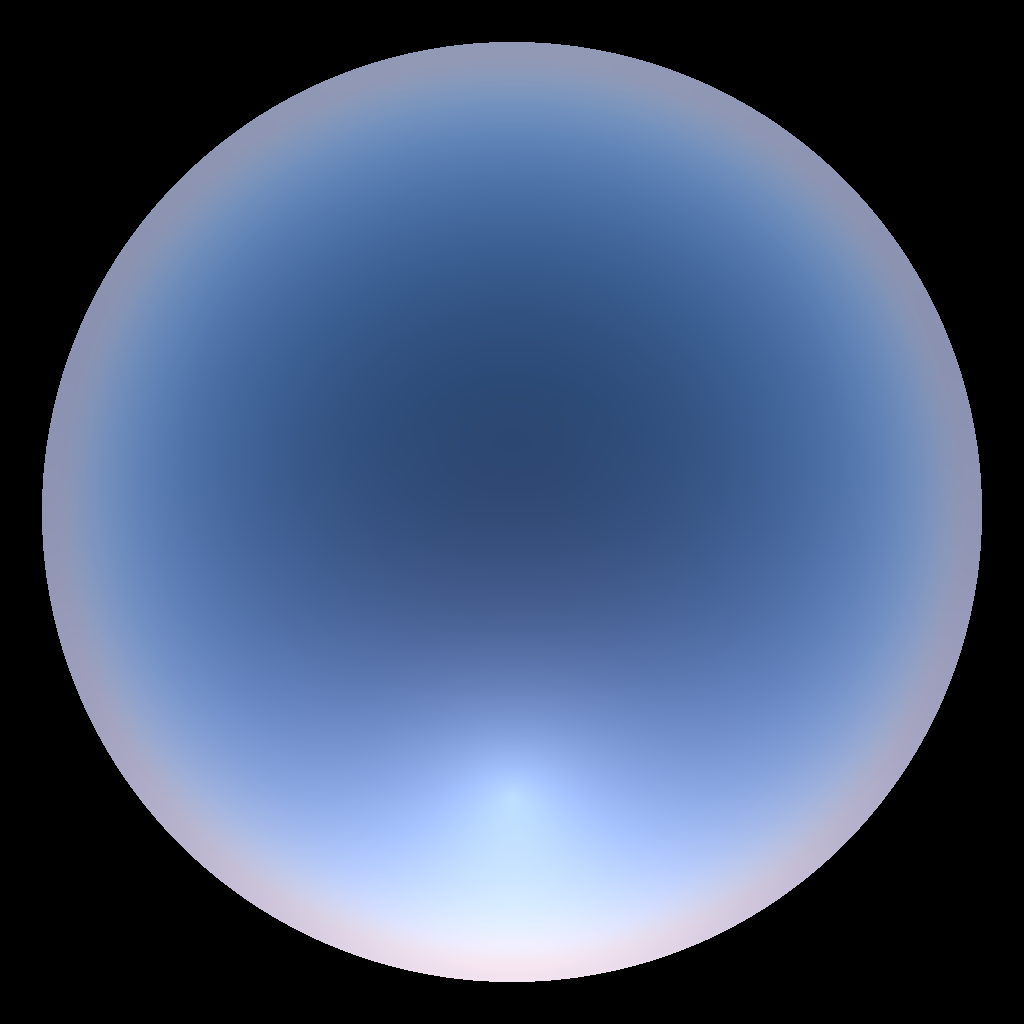
\includegraphics[scale=0.125]{figures/preetham_2.png}
 }
 \subtop
 {
 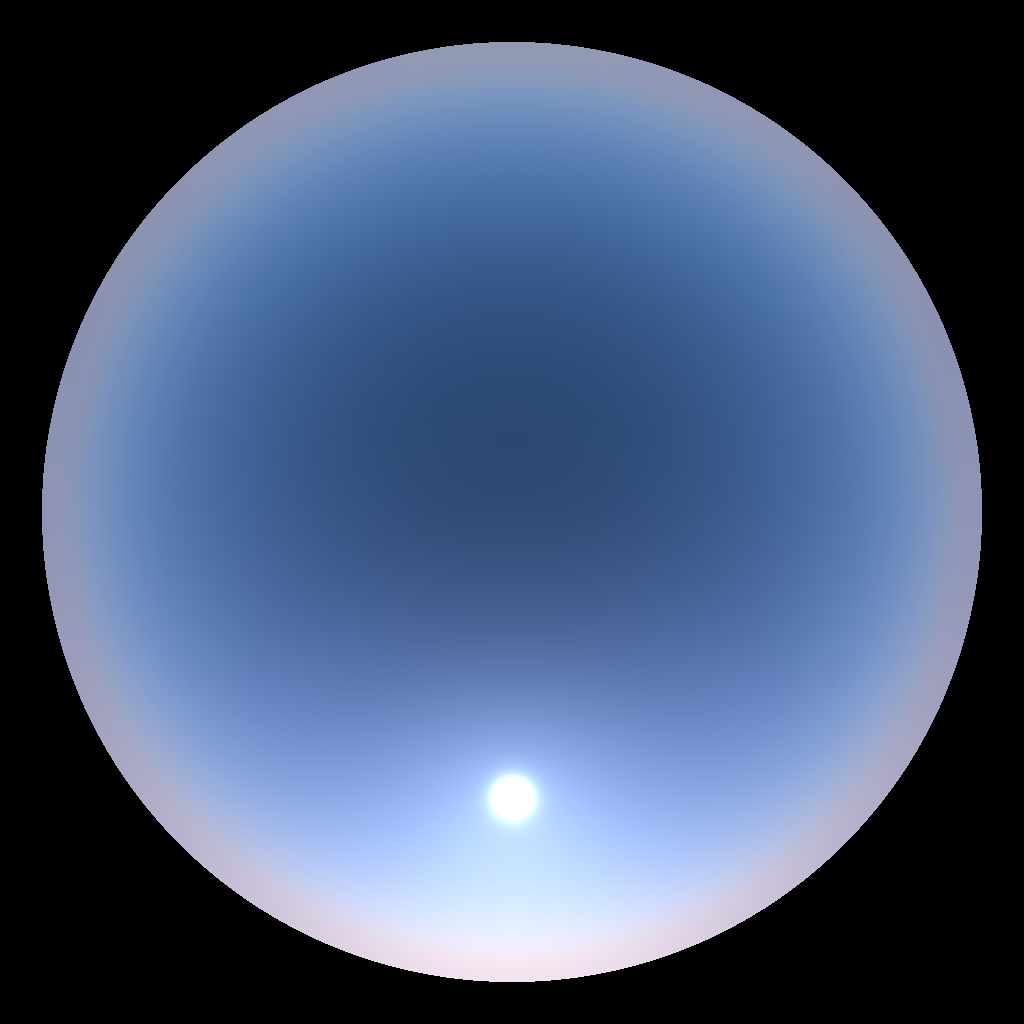
\includegraphics[scale=0.125]{figures/preetham_solar_disk_2.png}
 }
 \subtop
 {
 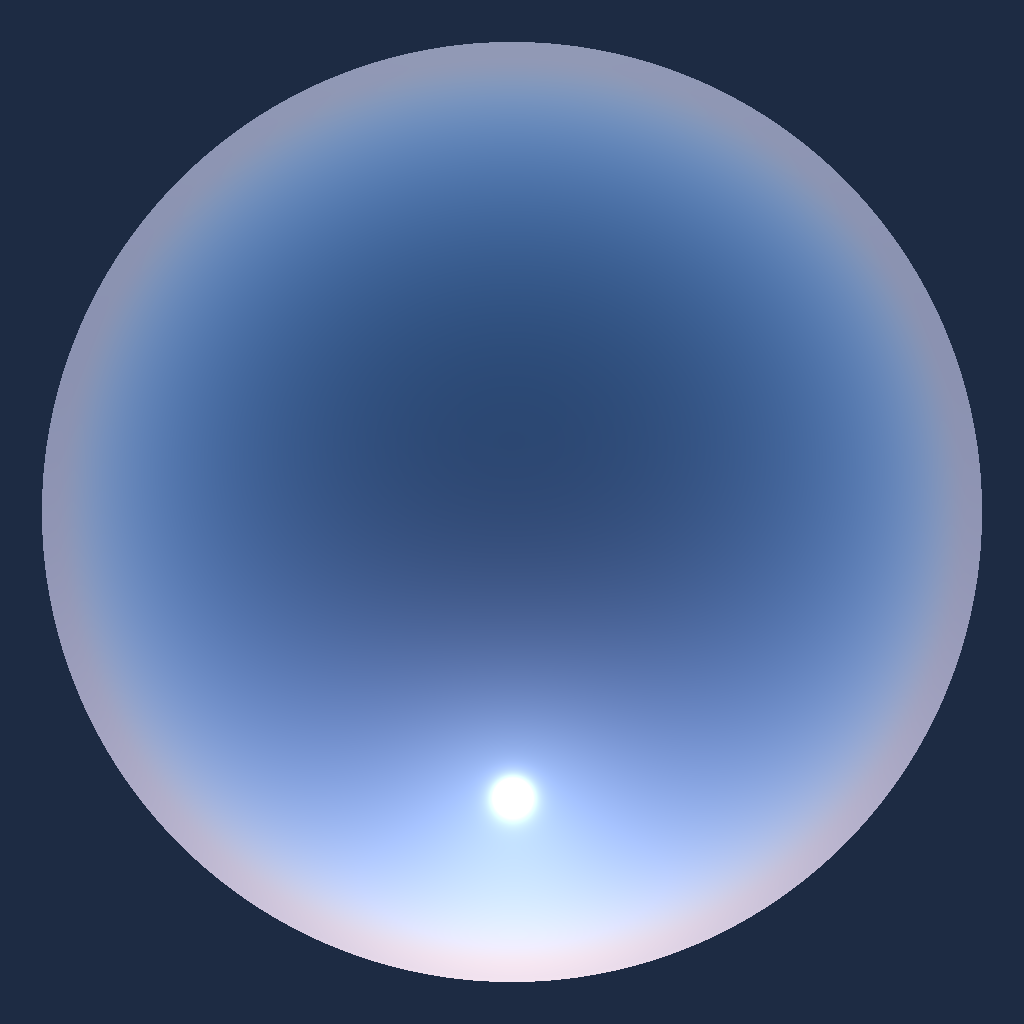
\includegraphics[scale=0.125]{figures/preetham_solar_disk_irradiance_2.png}
 }
 \subtop
 {
 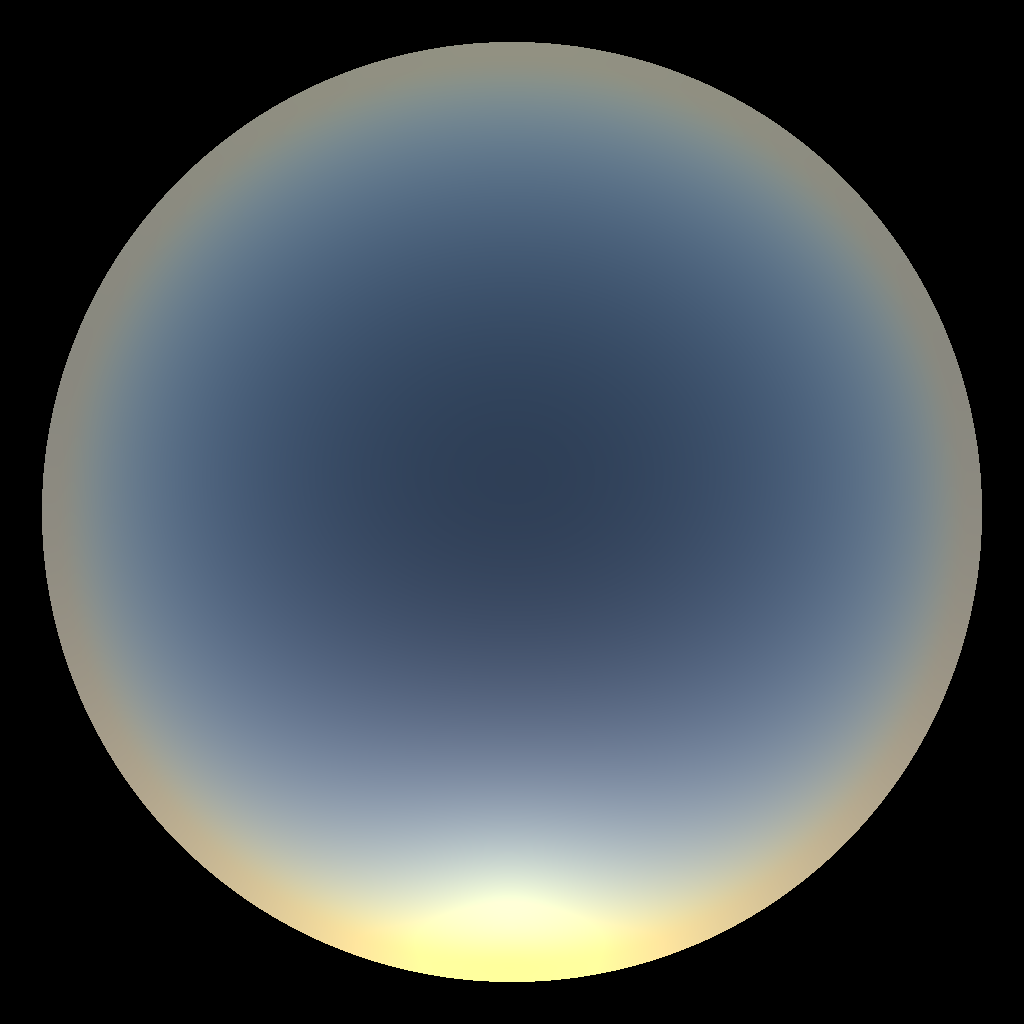
\includegraphics[scale=0.125]{figures/preetham_3.png}
 }
 \subtop
 {
 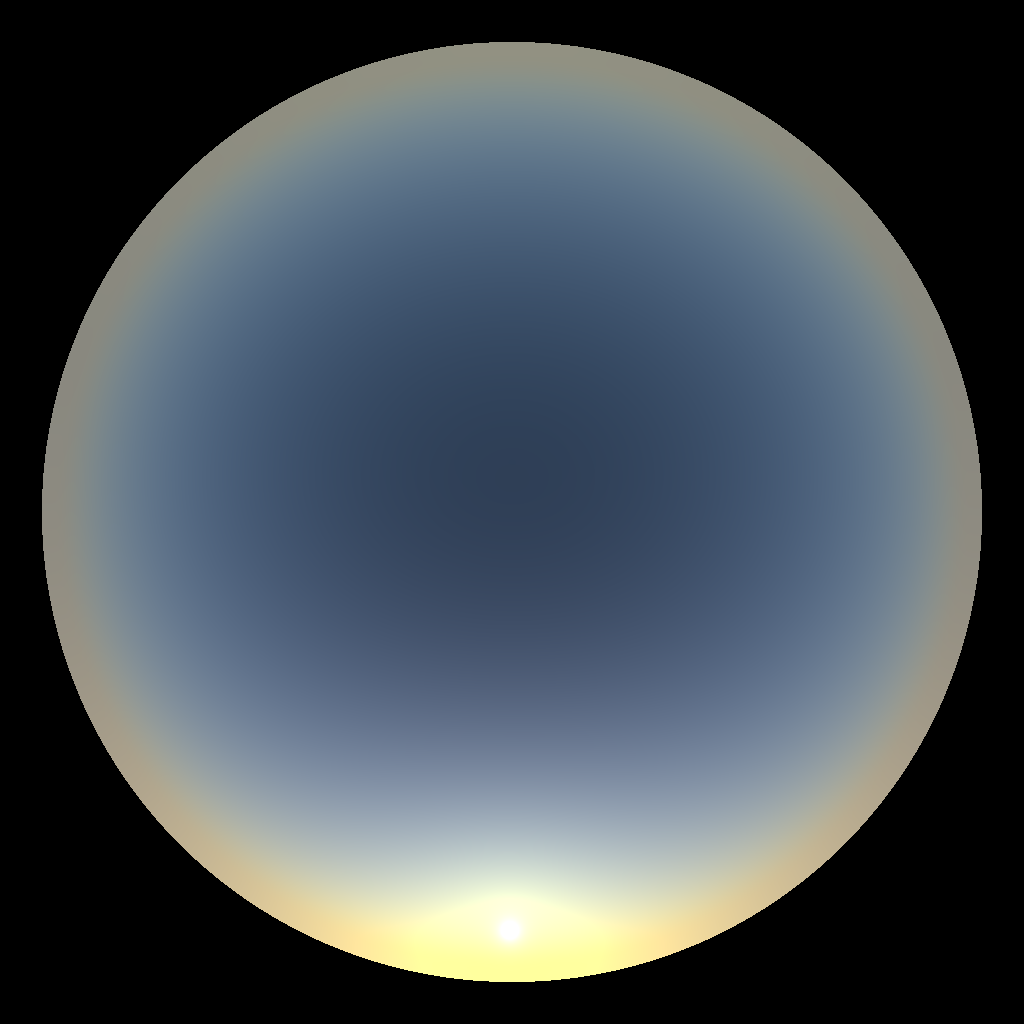
\includegraphics[scale=0.125]{figures/preetham_solar_disk_3.png}
 }
 \subtop
 {
 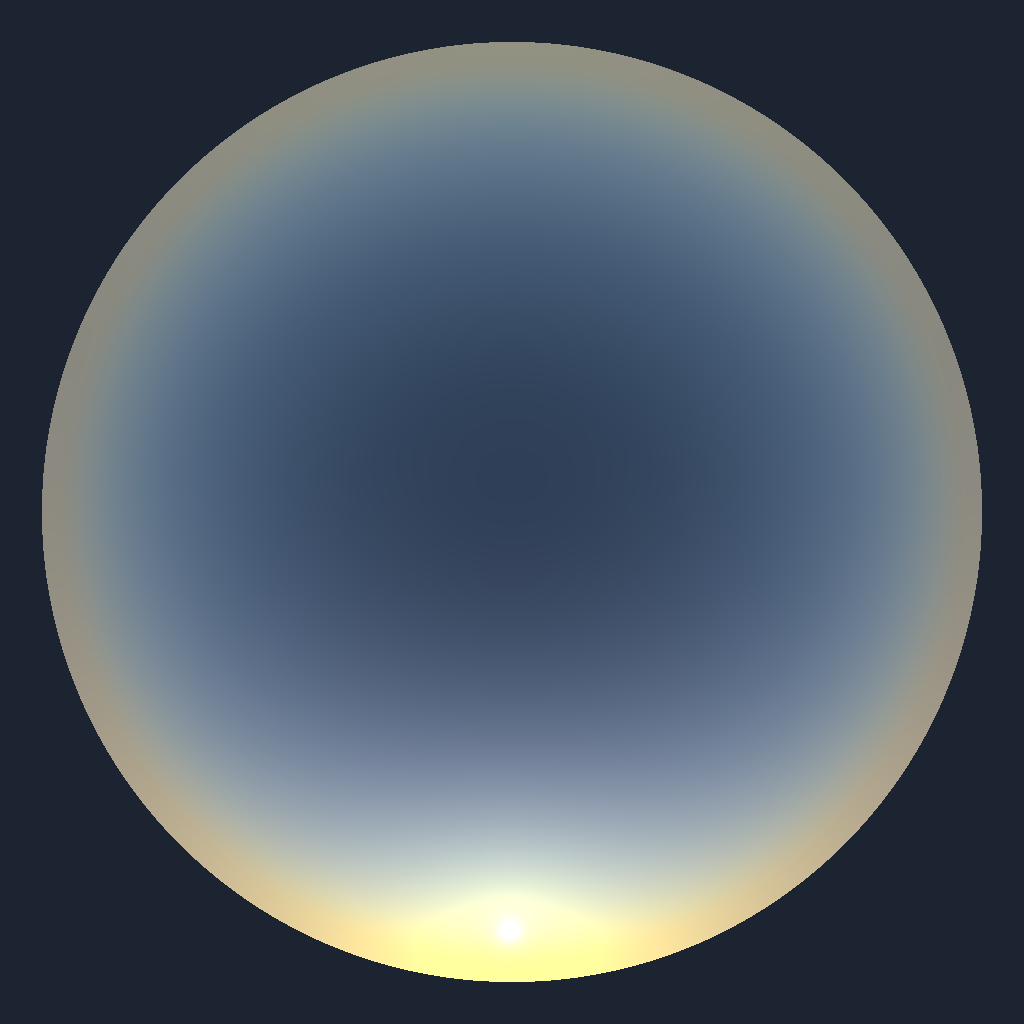
\includegraphics[scale=0.125]{figures/preetham_solar_disk_irradiance_3.png}
 }
\caption{Brak.}
\label{fig:preetham}
\end{figure}
%
\cite{Preetham:1999}
\subsubsection{Ocean Lighting}
\cite{article:oceanlighting}
\subsubsection{Whitecaps}
The ocean lighting scheme by Bruneton et al. \cite{article:oceanlighting} does
not account for the breaking of waves on the open ocean. Neither the geometric
deformations, nor the changes in reflectance caused by foam and spray, so called
\emph{whitecaps}, are incorporated in their model. Dupuy et al.\cite{article:whitecaps},
on the other hand, extend the FFT version of Bruneton et al.\cite{misc:oceanlightingfft}
to include whitecaps. Their work is based on Tessendorf's approach\cite{course:simulatingocean}
to locate self intersections on the ocean surface, see the discussion in Section~\ref{sec:self_intersections}. Given the location of a self intersection,
the reflectance at that position may be modified. Said modification is based on
the magnitude of the Jacobian determinant $det(\mvec{J}(\mvec{x},t))$ of the
horizontal displacement $\mvec{x}+u\mvec{D}(\mvec{x},t)$.

Dupuy et al. contribute  a GPU optimized version of the above. Their algorithm
requires an additional preprocessing step, where terms $k_i$ and $k_i^2$ from
Equation 7 and 8 in \cite{article:whitecaps} are precomputed, with the first
order partial derivatives of $\mvec{D}(\mvec{x},t)$ of all patterns as input.
%
\subsubsection{Tonemapping}
Rendering the Preetham sky and the ocean results in an image with a high dynamic range.
We need to map said image to the lower dynamic range of a standard monitor, by means
of a tonemapping operator. We chose Reinhard's global tonemapping operator, see
Equation 4 in\cite{Reinhard:2002}. It is straightforward to implement and
works well on the class of images the demo application renders. Note, that Equation 1
in\cite{Reinhard:2002} is incorrect, see\cite{Reinhard:2002:erratum}. The correct
form to compute the log-average luminance of an image is as follows:
\begin{equation*}
 \bar L_w = \exp\left(\frac{1}{N}\log(\delta + L_w(x,y))\right)
\end{equation*}
where $N$ is the number of pixels in the image, $L_w(x,y)$ is the ''world'' luminance for
pixel $(x,y)$, and $\delta$ is small positive value to avoid the singularity at
$\log(0)$. We compute $\bar L_w$ by simple means directly on the GPU. We employ a render
target the same size as the source image, where for each pixel of the source image
we compute $\log(\delta + L_w(x,y))$ and write it to the render target. We obtain
$L_w(x,y)$ by converting the source pixel's RGB color to CIE XYZ, and then using the
luminance component Y of the latter. Next, we generate the mipmap pyramid for
our render target. The highest mipmap level is one pixel in size and gives us
$\frac{1}{N}\log(\delta + L_w(x,y))$. Hence, we are able to get $\bar L_w$ by sampling
the highest mipmap level of our render target and then applying $\exp$ on the result.
